\documentclass[]{article}
\usepackage{lmodern}
\usepackage{amssymb,amsmath}
\usepackage{ifxetex,ifluatex}
\usepackage{fixltx2e} % provides \textsubscript
\ifnum 0\ifxetex 1\fi\ifluatex 1\fi=0 % if pdftex
  \usepackage[T1]{fontenc}
  \usepackage[utf8]{inputenc}
\else % if luatex or xelatex
  \ifxetex
    \usepackage{mathspec}
  \else
    \usepackage{fontspec}
  \fi
  \defaultfontfeatures{Ligatures=TeX,Scale=MatchLowercase}
\fi
% use upquote if available, for straight quotes in verbatim environments
\IfFileExists{upquote.sty}{\usepackage{upquote}}{}
% use microtype if available
\IfFileExists{microtype.sty}{%
\usepackage{microtype}
\UseMicrotypeSet[protrusion]{basicmath} % disable protrusion for tt fonts
}{}
\usepackage[margin=1in]{geometry}
\usepackage{hyperref}
\hypersetup{unicode=true,
            pdfborder={0 0 0},
            breaklinks=true}
\urlstyle{same}  % don't use monospace font for urls
\usepackage{longtable,booktabs}
\usepackage{graphicx,grffile}
\makeatletter
\def\maxwidth{\ifdim\Gin@nat@width>\linewidth\linewidth\else\Gin@nat@width\fi}
\def\maxheight{\ifdim\Gin@nat@height>\textheight\textheight\else\Gin@nat@height\fi}
\makeatother
% Scale images if necessary, so that they will not overflow the page
% margins by default, and it is still possible to overwrite the defaults
% using explicit options in \includegraphics[width, height, ...]{}
\setkeys{Gin}{width=\maxwidth,height=\maxheight,keepaspectratio}
\IfFileExists{parskip.sty}{%
\usepackage{parskip}
}{% else
\setlength{\parindent}{0pt}
\setlength{\parskip}{6pt plus 2pt minus 1pt}
}
\setlength{\emergencystretch}{3em}  % prevent overfull lines
\providecommand{\tightlist}{%
  \setlength{\itemsep}{0pt}\setlength{\parskip}{0pt}}
\setcounter{secnumdepth}{0}
% Redefines (sub)paragraphs to behave more like sections
\ifx\paragraph\undefined\else
\let\oldparagraph\paragraph
\renewcommand{\paragraph}[1]{\oldparagraph{#1}\mbox{}}
\fi
\ifx\subparagraph\undefined\else
\let\oldsubparagraph\subparagraph
\renewcommand{\subparagraph}[1]{\oldsubparagraph{#1}\mbox{}}
\fi

%%% Use protect on footnotes to avoid problems with footnotes in titles
\let\rmarkdownfootnote\footnote%
\def\footnote{\protect\rmarkdownfootnote}

%%% Change title format to be more compact
\usepackage{titling}

% Create subtitle command for use in maketitle
\providecommand{\subtitle}[1]{
  \posttitle{
    \begin{center}\large#1\end{center}
    }
}

\setlength{\droptitle}{-2em}

  \title{}
    \pretitle{\vspace{\droptitle}}
  \posttitle{}
    \author{}
    \preauthor{}\postauthor{}
    \date{}
    \predate{}\postdate{}
  
\usepackage[left]{lineno}
\linenumbers
\usepackage{setspace}
\doublespacing
\DeclareUnicodeCharacter{200E}{}
\usepackage{caption}
\captionsetup[figure]{labelformat=empty}
\captionsetup[table]{labelformat=empty}

\begin{document}

\section{Differential response of a tree-killing bark beetle to forest
structure across a gradient of climatic water
deficit}\label{differential-response-of-a-tree-killing-bark-beetle-to-forest-structure-across-a-gradient-of-climatic-water-deficit}

Michael J. Koontz\textsuperscript{1,2,*}, Andrew M.
Latimer\textsuperscript{1,2}, Leif A. Mortenson\textsuperscript{3},
Christopher J. Fettig\textsuperscript{3}, Malcolm P.
North\textsuperscript{1,2,4}

\textsuperscript{1}Graduate Group in Ecology, University of California,
Davis, CA, USA\\
\textsuperscript{2}Department of Plant Sciences, University of
California, Davis, CA, USA\\
\textsuperscript{3}USDA Forest Service, Pacific Southwest Research
Station, Placerville, CA, USA\\
\textsuperscript{4}USDA Forest Service, Pacific Southwest Research
Station, Davis, CA, USA

\textsuperscript{*}Correspondence: \texttt{michael.koontz@colorado.edu}

Date report generated: May 01, 2019

\subsection{Abstract}\label{abstract}

The recent Californian hot drought of 2012 to 2015 created favorable
conditions for unprecedented ponderosa pine mortality in the driest,
densest portions of the Sierra Nevada mountain range, largely caused by
the western pine beetle (\emph{Dendroctonus brevicomis}). Climate
conditions related to tree water stress as well as forest structure can
influence the severity of forest insect disturbance, but it remains
challenging to consider how these variables may interact to produce
patterns of tree mortality. Previous studies have shown an interaction
between climate conditions and forest density in their effect on tree
mortality, but density is a coarse gauge of forest structure that can
affect western pine beetle behavior in a number of ways. Measuring
broad-scale climate conditions simultaneously with complex forest
structure-- including tree species, tree size, and local density-- will
refine our understanding of how these variables interact, but is
generally expensive and/or labor-intensive. We overcame these hurdles by
using a small, unhumanned aerial system (hereafter `drone') to conduct
aerial surveys over an established network of 32 forest plots along a
350km and 1000m elevation gradient in western slope Sierra yellow
pine/mixed-conifer forests. Using Structure from Motion (SfM) processing
on over 450,000 images and field measurements from the coincident ground
plots, we determined tree size, location, and species for individual
trees over 9 square kilometers of forest that experienced ponderosa pine
mortality as a result of western pine beetle activity. We modeled the
probability of ponderosa pine mortality as a linear combination of
forest structure variables and site-level climatic water deficit, and
used a Gaussian process to estimate the spatial covariance in the
response.

We found that greater host density strongly increased the probability of
host mortality, and greater host size generally decreased the
probability of host mortality. There was also a strong three-way
interaction between host density, host size, and climatic water deficit
such that host density and host size tended to synergistically increase
the probability of host mortality at hot/dry sites, but denser, smaller
trees tended to drive mortality in cool/wet sites.

Our results demonstrate a variable response of the western pine beetle
to complex forest structure across an environmental gradient during the
same hot drought, which may indicate forest sites were in different
stages of disturbance (from ``endemic'' to ``outbreak'') depending on
their regional climate. Management interventions that reduce stem
density may decrease the severity of western pine beetle disturbance in
the future, and our results suggest that focusing these treatments on
areas that are most likely to exceed feedback thresholds (i.e., hot/dry
sites with many available hosts) will have the best chance of increasing
the survivorship probability of larger trees.

\subsection{Introduction}\label{introduction}

Aggressive bark beetles dealt the final blow to many of the nearly 150
million trees killed in the California hot drought of 2012 to 2015 and
its aftermath (USDAFS 2019). A harbinger of climate change effects to
come, record high temperatures exacerbated the drought (Griffin and
Anchukaitis 2014), which increased water stress on trees (Asner et al.
2016), making them more susceptible to attacking bark beetles (Fettig
2012, Kolb et al. 2016). A century of fire suppression policy has
enabled forests to grow into dense stands, which also makes them more
vulnerable to bark beetle attack (Fettig 2012). This combination of
environmental conditions and forest structural characteristics led to
tree mortality events of unprecedented size in the driest, densest
forests across the state (Young et al. 2017). The mechanisms underlying
the link between tree susceptibility to insect attack and hot, dry
conditions are often directly attributed to tree physiology (Bentz et
al. 2010), while the link to forest density is multifaceted (Fettig
2012). Because forest density is a coarse metric of the complex forest
structure to which bark beetles respond (Raffa et al. 2008), our
understanding of the connection between forest density and insect
disturbance severity could be enhanced with more finely-resolved
measures of forest structure, such as tree size, tree species, and local
density within a forest stand (Stephenson et al. 2019, Fettig et al.
2019). Further, the interaction between local-scale complex forest
structure and broad-scale environmental conditions as they affect forest
insect disturbance remains underexplored (Seidl et al. 2016, Stephenson
et al. 2019, Fettig et al. 2019).

The yellow pine/mixed-conifer forests in California's Sierra Nevada
region are characterized by regular bark beetle disturbances, primarily
by the western pine beetle (\emph{Dentrodctonus brevicomis}) and its
main host in the system, ponderosa pine (\emph{Pinus ponderosa}) (Fettig
et al. 2019). The western pine beetle is a ``primary'' or ``aggressive''
bark beetle, with reproductive success contingent upon enough beetles
``mass attacking'' the host tree, overwhelming its defenses, and causing
mortality (Raffa and Berryman 1983, Fettig et al. 2019). This Allee
effect creates a strong coupling between beetle host selection behavior
and host tree susceptibility to attack (Raffa and Berryman 1983, Logan
et al. 1998). Under normal conditions, weakened trees are the most
susceptible to attack and will be the main targets of aggressive bark
beetles like the western pine beetle (Bentz et al. 2010, Raffa et al.
2015). A key defense mechanism of trees to bark beetle attack is to
flood beetle bore holes with resin, which physically expels beetles and
may interrupt beetle communication (Raffa et al. 2015). Under severe
water stress, trees no longer have the resources available to mount this
defense (Kolb et al. 2016) and thus prolonged drought can often trigger
increased bark beetle-induced tree mortality as average tree vigor
declines (Bentz et al. 2010). As local beetle density increases due to
successful reproduction on spatially-aggregated weakened trees, as might
occur in a prolonged drought, mass attacks become capable of
overwhelming any tree's defenses and even healthy trees become
susceptible (Bentz et al. 2010, Raffa et al. 2015). Thus, water stress
can be a key determinant of whether individual trees are susceptible to
bark beetle attack under many conditions, and this environmental
condition may interact with other forest features, such as tree size, to
drive susceptibility under extreme conditions (Bentz et al. 2010,
Stephenson et al. 2019).

Forest structure-- often characterized as the spatial distribution,
size, and species composition of trees-- also strongly influences
western pine beetle activity. For instance, high-density forests are
more prone to bark beetle attacks, and several mechanism likely underlie
this phenomenon (Fettig 2012). A high-density forest may experience
greater bark beetle-induced tree mortality for several reasons
including: a) host availability is high and shorter dispersal distances
facilitate successful colonization of those hosts (Miller and Keen 1960,
Berryman 1982, Fettig et al. 2007); b) high host availability reduces
the chance of individual beetles wasting their limited resources flying
to and landing on a non-host tree (Moeck et al. 1981, Evenden et al.
2014); c) crowded trees experience greater competition for water
resources and thus average tree resistance is lower (Hayes et al. 2009);
or d) smaller gaps between trees protect pheromone plumes from
dissipation by the wind and thus enhance intraspecific beetle
communication (Thistle et al. 2004). Additionally, tree size affects
bark beetle host selection behavior as smaller trees tend to have less
capacity for resisting attack, but larger trees represent a more
desirable target because their thicker phloem provides greater
nutritional value (Chubaty et al. 2009, Graf et al. 2012). Tree density
thus paints a fundamentally limited picture of the mechanism by which
forest structure affects bark beetle disturbance, but \emph{complex}
forest structure-- with explicit recognition of tree size, species
composition (e.g., host versus non-host composition), and local tree
density-- should more appropriately capture the ecological processes
underlying insect-induced tree mortality. Additionally, considering the
effects of complex forest structure simultaneously to the effects of
environmental conditions may help refine our understanding of observed
patterns of tree mortality in the recent California hot drought.

The vast spatial extent of tree mortality in the 2012 to 2015 California
hot drought (USDAFS 2019) challenges our ability to simultaneously
consider how broad-scale environmental conditions may interact with
local, complex forest structure to affect the dynamic between bark
beetle host selection and host tree susceptibility to attack (Anderegg
et al. 2015, Stephenson et al. 2019). Measuring complex forest structure
generally requires expensive instrumentation (Kane et al. 2014, Asner et
al. 2016) or labor-intensive field surveys (Larson and Churchill 2012,
Stephenson et al. 2019), which constrains survey extent and frequency.
Small, unhumanned aerial systems (sUAS) enable relatively fast and cheap
remote imaging over dozens of hectares of forest, which can be used to
measure complex forest structure at the individual tree scale (Morris et
al. 2017, Shiklomanov et al. 2019). Distributing such surveys across an
environmental gradient is a viable approach to overcoming the data
acquisition challenge inherent in investigating phenomena with both a
strong local- and a strong broad-scale component.

We used ultra-high resolution, drone-derived remote sensing data over a
network of 32 sites in Sierra Nevada yellow pine/mixed-conifer forests
spanning 1000m of elevation and 350km of latitude and covering a total
of 9 square kilometers to ask how broad-scale environmental conditions
interacted with local, complex forest structure to affect the
probability of tree mortality during the cumulative tree mortality event
of 2012 to 2018. We asked:

\begin{enumerate}
\def\labelenumi{\arabic{enumi}.}
\item
  How does host tree density and average host tree size affect the
  severity of western pine beetle disturbance?
\item
  How does tree density of all species (hereafter ``overall density'')
  and average tree size of all species (hereafter ``overall size'')
  affect the severity of western pine beetle disturbance?
\item
  How does environmentally-driven tree moisture stress affect the
  severity of western pine beetle disturbance?
\item
  Do the effects of forest structure and environmental condition on
  western pine beetle disturbance interact?
\end{enumerate}

\subsection{Methods}\label{methods}

\subsubsection{Study system}\label{study-system}

\begin{figure}
\centering
\includegraphics[height=7.00000in]{../../figures/study-geographic-extent-inset.png}
\caption{Figure 1: The network of field plots spanned a 350 km
latitudinal gradient from the Eldorado National Forest in the north to
the Sequoia National Forest in the south. Plots were stratified by three
elevation bands in each forest, with the plots in the Sequoia National
Forest (the southern-most National Forest) occupying elevation bands
305m above the three bands in the other National Forests in order to
capture a similar community composition.}
\end{figure}

The study sites were chosen to reflect typical west-side Sierra Nevada
yellow pine/mixed-conifer forests and were dominated by ponderosa pine
trees, \emph{Pinus ponderosa} (Fettig et al. 2019), whose primary bark
beetle predator in California is the western pine beetle (WPB),
\emph{Dendroctonus brevicomis}. The typical life cycle of WPBs consists
of pioneer beetles dispersing to a new host tree, determining the host's
susceptibility to attack, and using pheromone signals to attract other
WPBs. The attracted WPBs mass attack the tree by boring into its inner
bark, laying eggs, and dying, leaving their offspring to develop inside
the doomed tree before themselves dispersing to a new potential host
(Raffa et al. 2008). In California, the WPB can have 2-3 generations in
a single year and can often out-compete its congener, the mountain pine
beetle, \emph{Dendroctonus ponderosa} (MPB), for the ponderosa pine host
(Fettig et al. 2019).

We built our study on 180 vegetation/forest insect monitoring plots at
36 sites established between 2016 and 2017 by Fettig et al. (2019)
(Figure 1). These established plots were located in WPB-attacked, yellow
pine/mixed-conifer forests across the Eldorado, Stanislaus, Sierra and
Sequoia National Forests and were stratified by elevation (914-1219
meters {[}3000-4000 feet{]}, 1219-1524 meters {[}4000-5000 feet{]},
1524-1828 meters {[}5000-6000 feet{]} above sea level). In the Sequoia
National Forest, the southernmost National Forest in our study, plots
were stratified with the lowest elevation band between 1219 and 1524
meters (4000-5000 feet) and extended to an upper elevation band of
1828-2133 meters (6000-7000 feet) to capture a more similar forest
community composition as at the more northern National Forests. The
sites have variable forest structure and plot locations were selected in
areas with \textgreater{}40\% ponderosa pine basal area and
\textgreater{}10\% ponderosa pine mortality. At each site, five 0.04 ha
circular plots were installed along transects with between 80 and 200m
between each plot. In the field, Fettig et al. (2019) mapped all stem
locations relative to the center of each plot using azimuth/distance
measurements. Tree identity to species, tree height, and diameter at
breast height (DBH) were recorded if DBH was greater than 6.35cm. Year
of mortality was estimated based on needle color and retention, if it
wasn't directly observed between site visits. A small section of bark
was removed from dead trees to confirm insect activity. During the
spring and early summer of 2018, all field plots were revisited to
assess whether dead trees had fallen (Fettig et al. 2019).

\subsubsection{Instrumentation}\label{instrumentation}

Imagery was captured using a DJI Zenmuse X3 RGB camera (DJI 2015a) and a
Micasense RedEdge3 5-band multispectral camera (Micasense 2015). We
mounted both of these instruments simultaneously on a DJI Matrice 100
aircraft (DJI 2015b) using the DJI 3-axis stabilized gimbal for the
Zenmuse X3 camera and a Micasense angled fixed mount for the RedEdge3
camera. The gimbal and the angled fixed mount ensured both instruments
were nadir-facing during image capture. Just prior to or after image
capture at each site, we calibrated the RedEdge3 camera by taking an
image of a calibration panel on the ground in full sun with known
reflectance values for each of the 5 narrow bands (Table 1).

\begin{longtable}[]{@{}cccccc@{}}
\caption{Table 1: Reflectance sensitivity of the Micasense Rededge3
camera. The calibration panel value represents the reflectance of the
calibration panel for the given wavelength.}\tabularnewline
\toprule
\begin{minipage}[b]{0.10\columnwidth}\centering\strut
Band number\strut
\end{minipage} & \begin{minipage}[b]{0.23\columnwidth}\centering\strut
Band name\strut
\end{minipage} & \begin{minipage}[b]{0.14\columnwidth}\centering\strut
Center wavelength\strut
\end{minipage} & \begin{minipage}[b]{0.09\columnwidth}\centering\strut
Band width\strut
\end{minipage} & \begin{minipage}[b]{0.14\columnwidth}\centering\strut
Wavelength range\strut
\end{minipage} & \begin{minipage}[b]{0.14\columnwidth}\centering\strut
Panel reflectance\strut
\end{minipage}\tabularnewline
\midrule
\endfirsthead
\toprule
\begin{minipage}[b]{0.10\columnwidth}\centering\strut
Band number\strut
\end{minipage} & \begin{minipage}[b]{0.23\columnwidth}\centering\strut
Band name\strut
\end{minipage} & \begin{minipage}[b]{0.14\columnwidth}\centering\strut
Center wavelength\strut
\end{minipage} & \begin{minipage}[b]{0.09\columnwidth}\centering\strut
Band width\strut
\end{minipage} & \begin{minipage}[b]{0.14\columnwidth}\centering\strut
Wavelength range\strut
\end{minipage} & \begin{minipage}[b]{0.14\columnwidth}\centering\strut
Panel reflectance\strut
\end{minipage}\tabularnewline
\midrule
\endhead
\begin{minipage}[t]{0.10\columnwidth}\centering\strut
1\strut
\end{minipage} & \begin{minipage}[t]{0.23\columnwidth}\centering\strut
blue (b)\strut
\end{minipage} & \begin{minipage}[t]{0.14\columnwidth}\centering\strut
475\strut
\end{minipage} & \begin{minipage}[t]{0.09\columnwidth}\centering\strut
20\strut
\end{minipage} & \begin{minipage}[t]{0.14\columnwidth}\centering\strut
465-485\strut
\end{minipage} & \begin{minipage}[t]{0.14\columnwidth}\centering\strut
0.64\strut
\end{minipage}\tabularnewline
\begin{minipage}[t]{0.10\columnwidth}\centering\strut
2\strut
\end{minipage} & \begin{minipage}[t]{0.23\columnwidth}\centering\strut
green (g)\strut
\end{minipage} & \begin{minipage}[t]{0.14\columnwidth}\centering\strut
560\strut
\end{minipage} & \begin{minipage}[t]{0.09\columnwidth}\centering\strut
20\strut
\end{minipage} & \begin{minipage}[t]{0.14\columnwidth}\centering\strut
550-570\strut
\end{minipage} & \begin{minipage}[t]{0.14\columnwidth}\centering\strut
0.64\strut
\end{minipage}\tabularnewline
\begin{minipage}[t]{0.10\columnwidth}\centering\strut
3\strut
\end{minipage} & \begin{minipage}[t]{0.23\columnwidth}\centering\strut
red (r)\strut
\end{minipage} & \begin{minipage}[t]{0.14\columnwidth}\centering\strut
668\strut
\end{minipage} & \begin{minipage}[t]{0.09\columnwidth}\centering\strut
10\strut
\end{minipage} & \begin{minipage}[t]{0.14\columnwidth}\centering\strut
663-673\strut
\end{minipage} & \begin{minipage}[t]{0.14\columnwidth}\centering\strut
0.64\strut
\end{minipage}\tabularnewline
\begin{minipage}[t]{0.10\columnwidth}\centering\strut
4\strut
\end{minipage} & \begin{minipage}[t]{0.23\columnwidth}\centering\strut
near infrared (nir)\strut
\end{minipage} & \begin{minipage}[t]{0.14\columnwidth}\centering\strut
840\strut
\end{minipage} & \begin{minipage}[t]{0.09\columnwidth}\centering\strut
40\strut
\end{minipage} & \begin{minipage}[t]{0.14\columnwidth}\centering\strut
820-860\strut
\end{minipage} & \begin{minipage}[t]{0.14\columnwidth}\centering\strut
0.6\strut
\end{minipage}\tabularnewline
\begin{minipage}[t]{0.10\columnwidth}\centering\strut
5\strut
\end{minipage} & \begin{minipage}[t]{0.23\columnwidth}\centering\strut
red edge (re)\strut
\end{minipage} & \begin{minipage}[t]{0.14\columnwidth}\centering\strut
717\strut
\end{minipage} & \begin{minipage}[t]{0.09\columnwidth}\centering\strut
10\strut
\end{minipage} & \begin{minipage}[t]{0.14\columnwidth}\centering\strut
712-722\strut
\end{minipage} & \begin{minipage}[t]{0.14\columnwidth}\centering\strut
0.63\strut
\end{minipage}\tabularnewline
\bottomrule
\end{longtable}

\subsubsection{Flight protocol}\label{flight-protocol}

Image capture was conducted as close to solar noon as possible to
minimize shadow effects (varying primarily due to site accessibility;
always within 4 hours, usually within 2 hours). Prior to the aerial
survey, two strips of bright orange drop cloth (\textasciitilde{}100cm x
15cm) were positioned as an ``X'' over the permanent monuments marking
the center of the 5 field plots from Fettig et al. (2019).

For each of the 36 sites (containing 5 plots each), we captured imagery
over the surrounding \textasciitilde{}40 hectares of forested area using
north-south aerial transects. For three sites, we surveyed less
surrounding area in order to maintain visual and radio communication
with the aircraft during flight which can be obstructed by rolling
terrain or non-centrally available takeoff locations.

We preprogrammed aerial transects using Map Pilot for DJI on iOS flight
software (hereafter Map Pilot) (DronesMadeEasy 2018). Using the Map
Pilot software, we included an altitude adjustment along each aerial
transect using a 1-arc-second digital elevation model (Farr et al. 2007)
such that the aircraft's altitude remained approximately constant at 120
meters above ground level in order to maintain consistent ground
sampling distance (centimeters on the ground per pixel) in the imagery.
Ground sampling distance was approximately 5 cm/px for the Zenmuse X3
RGB camera and approximately 8 cm/px for the RedEdge3 multispectral
camera. For this analysis, we dropped 4 sites whose imagery was of
insufficient quality to process.

Structure from motion (SfM) processing requires highly overlapping
images, especially in densely vegetated areas (Frey et al. 2018). We
planned transects with 90\% forward overlap and 90\% side overlap at 100
meters below the lens. Thus, with flights being at 120 meters above
ground level, we achieved slightly higher than 90/90\% overlap for
objects under 20 meters tall (91.6/91.6\% overlap at the ground).
Overlap values were based on focal length (3.6mm), sensor width (6.2mm),
and image dimension (4000x3000 pixels) parameters of the Zenmuse X3
camera. Images were captured at a constant rate of 1 image every 2
seconds for both cameras. A forward overlap of 90\% at 100 meters
translates to a flight speed of approximately 6.45 m/s and a side
overlap of 90\% at 100 meters translates to transects approximately 17.2
meters apart. The RedEdge3 camera has a different focal length (5.4mm),
sensor width (4.8mm), and image dimension (1280x960 pixels), which
translates to image overlap of 80.7/80.7 \% at 100m below the lens and
83.9/83.9 \% at ground level. Approximately 1900 photos were captured
over each 40 hectare survey area for each camera.

\subsubsection{Structure from Motion (SfM)
processing}\label{structure-from-motion-sfm-processing}

We used structure from motion (SfM) to generate dense point clouds
(Figure 2), digital surface models (Figure 3), and orthorectified
reflectance maps (Figure 4) for each field site (Frey et al. 2018). We
used Pix4Dmapper Cloud to process imagery using parameters ideal for
images of a densely vegetated area taken by a multispectral camera. For
29 sites, we processed the RedEdge3 multispectral imagery alone. For
three sites, we processed the RGB and the multispectral imagery in the
same project to enhance the point density of the resulting point cloud.
All SfM projects resulted in a single processing ``block,'' indicating
that all images in the project were optimized and processed together.

\begin{figure}
\centering
\includegraphics{../../figures/eldo_3k_3_point_cloud.png}
\caption{Figure 2: A dense point cloud representing \textasciitilde{}40
hectares of forest is generated using Structure from Motion (SfM)
processing of \textasciitilde{}1900 images. The dense point cloud z-
position represents the ground elevation plus the vegetation height.}
\end{figure}

\begin{figure}
\centering
\includegraphics{../../figures/eldo_3k_3_dsm.png}
\caption{Figure 3: The digital surface model (DSM) is a 2-dimensional
representation of the dense point cloud generated using structure from
motion (SfM) processing. The DSM represents the ground elevation plus
the vegetation height.}
\end{figure}

\begin{figure}
\centering
\includegraphics{../../figures/eldo_3k_3_2_ortho-rgb.png}
\caption{Figure 4: The orthomosaic for each of the 32 sites is generated
with the Structure from Motion (SfM) processing, showing a top-down view
of the whole survey area such that distances between objects in the
scene are preserved and can be measured. Depicted is an example
orthomosaic for one of the 32 sites cropped to the extent of a single
ground plot (5 ground plots per site) showing the orange X placed at
exactly the plot center prior to flight. The original orthomosaic for
the whole site represents an area approximately 1000 times as large as
the area depicted here.}
\end{figure}

\subsubsection{Creating canopy height
models}\label{creating-canopy-height-models}

\begin{figure}
\centering
\includegraphics{../../figures/eldo_3k_3_dtm.png}
\caption{Figure 5: The digital terrain model (DTM) is generated by
processing the dense point cloud using the cloth simulation filter
algorithm (Zhang et al. 2016), which classifies points as `ground' or
`not-ground' and then interpolates the `ground' elevation using Delaunay
triangulation for the rest of the dense point cloud footprint. The DTM
represents the ground elevation without any vegetation.}
\end{figure}

\begin{figure}
\centering
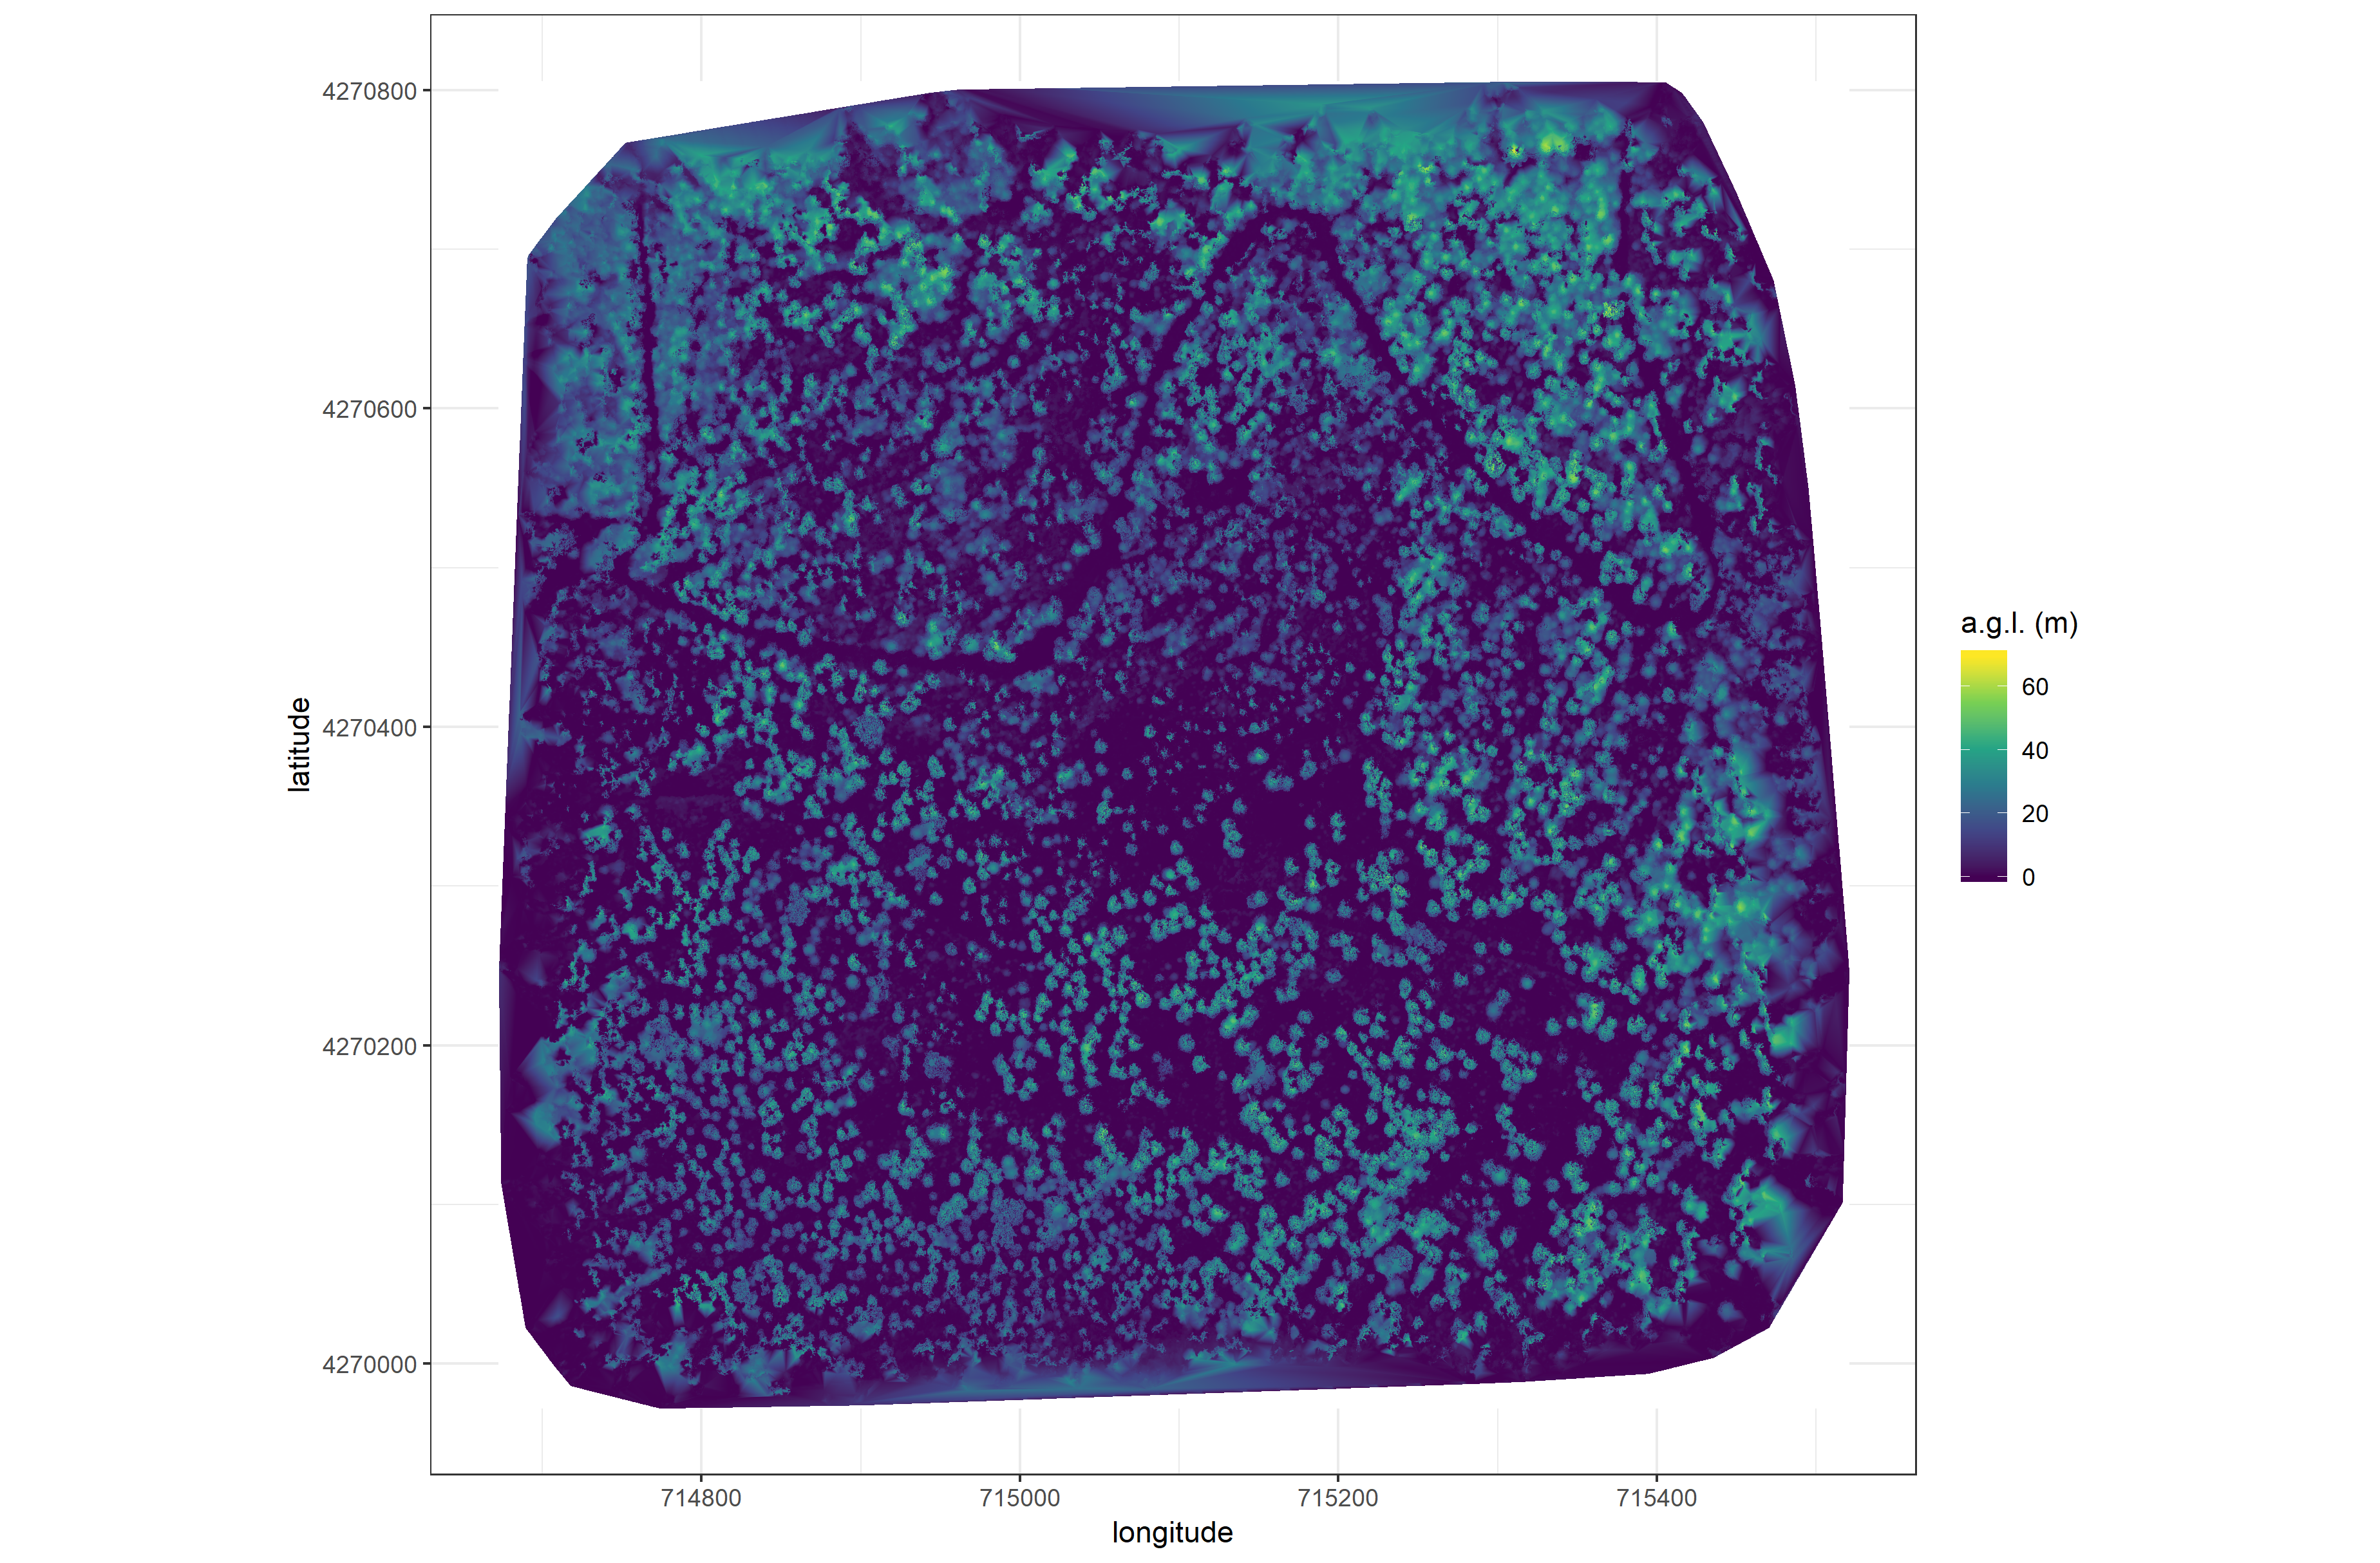
\includegraphics{../../figures/eldo_3k_3_chm.png}
\caption{Figure 6: The canopy height model (CHM) is generated by
subtracting the digital terrain model from the digital surface model.
The CHM represents the height of all of the elevation above ground
level.}
\end{figure}

We classified each survey area's dense point cloud into ``ground'' and
``non-ground'' points using a cloth simulation filter algorithm (Zhang
et al. 2016) implemented in the \texttt{lidR} (Roussel et al. 2019)
package. We rasterized the ground points using the \texttt{raster}
package (Hijmans et al. 2019) to create a digital terrain model (Figure
5) representing the ground underneath the vegetation at 1 meter
resolution. We created a canopy height model (Figure 6) by subtracting
the digital terrain model from the digital surface model created in
Pix4Dmapper.

\subsubsection{Tree detection}\label{tree-detection}

We tested a total of 7 automatic tree detection algorithms and a total
of 177 parameter sets on the canopy height model or the dense point
cloud to locate trees within each site (Table 2). We used 3 parameter
sets of a variable window filter using the \texttt{vwf()} function in
the \texttt{ForestTools} (Plowright 2018) \texttt{R} package, including
the default \texttt{winFun} parameter for the \texttt{vwf()} function as
well as the ``pines'' and ``combined'' functions from Popescu and Wynne
(2004) as the \texttt{winFun} parameter. We used 6 parameter sets of a
local maximum filter implemented in \texttt{lidR}. We used 131 parameter
sets of the algorithm from Li et al. (2012), which operates on the
original point cloud. These parameter sets included those from Shin et
al. (2018) and Jakubowski et al. (2013). We used 3 parameter sets of the
\texttt{watershed} algorithm implemented in \texttt{lidR}, which is a
wrapper for a function in the \texttt{EBImage} package (Pau et al.
2010). We used 3 parameter sets of \texttt{ptrees} (Vega et al. 2014)
implemented in \texttt{lidR} (Roussel et al. 2019) and
\texttt{lidRplugins} (Roussel 2019) and which operates on the raw point
cloud, without first normalizing it to height above ground level (i.e..
subtracting the ground elevation from the dense point cloud). We used
the default parameter set of the \texttt{multichm} (Eysn et al. 2015)
algorithm implemented in \texttt{lidR} (Roussel et al. 2019) and
\texttt{lidRplugins} (Roussel 2019). Finally, we used 30 parameter sets
of the experimental algorithm \texttt{lmfx} (Roussel 2019).

\begin{longtable}[]{@{}ccc@{}}
\caption{Table 2: Algorithm name, number of parameter sets tested for
each algorithm, and references.}\tabularnewline
\toprule
\begin{minipage}[b]{0.18\columnwidth}\centering\strut
Algorithm\strut
\end{minipage} & \begin{minipage}[b]{0.22\columnwidth}\centering\strut
Parameter sets tested\strut
\end{minipage} & \begin{minipage}[b]{0.34\columnwidth}\centering\strut
Reference(s)\strut
\end{minipage}\tabularnewline
\midrule
\endfirsthead
\toprule
\begin{minipage}[b]{0.18\columnwidth}\centering\strut
Algorithm\strut
\end{minipage} & \begin{minipage}[b]{0.22\columnwidth}\centering\strut
Parameter sets tested\strut
\end{minipage} & \begin{minipage}[b]{0.34\columnwidth}\centering\strut
Reference(s)\strut
\end{minipage}\tabularnewline
\midrule
\endhead
\begin{minipage}[t]{0.18\columnwidth}\centering\strut
li2012\strut
\end{minipage} & \begin{minipage}[t]{0.22\columnwidth}\centering\strut
131\strut
\end{minipage} & \begin{minipage}[t]{0.34\columnwidth}\centering\strut
Li et al. (2012); Jakubowski et al. (2013); Shin et al. (2018)\strut
\end{minipage}\tabularnewline
\begin{minipage}[t]{0.18\columnwidth}\centering\strut
lmfx\strut
\end{minipage} & \begin{minipage}[t]{0.22\columnwidth}\centering\strut
30\strut
\end{minipage} & \begin{minipage}[t]{0.34\columnwidth}\centering\strut
Roussel (2019)\strut
\end{minipage}\tabularnewline
\begin{minipage}[t]{0.18\columnwidth}\centering\strut
localMaxima\strut
\end{minipage} & \begin{minipage}[t]{0.22\columnwidth}\centering\strut
6\strut
\end{minipage} & \begin{minipage}[t]{0.34\columnwidth}\centering\strut
Roussel et al. (2019)\strut
\end{minipage}\tabularnewline
\begin{minipage}[t]{0.18\columnwidth}\centering\strut
multichm\strut
\end{minipage} & \begin{minipage}[t]{0.22\columnwidth}\centering\strut
1\strut
\end{minipage} & \begin{minipage}[t]{0.34\columnwidth}\centering\strut
Eysn et al. (2015)\strut
\end{minipage}\tabularnewline
\begin{minipage}[t]{0.18\columnwidth}\centering\strut
ptrees\strut
\end{minipage} & \begin{minipage}[t]{0.22\columnwidth}\centering\strut
3\strut
\end{minipage} & \begin{minipage}[t]{0.34\columnwidth}\centering\strut
Vega et al. (2014)\strut
\end{minipage}\tabularnewline
\begin{minipage}[t]{0.18\columnwidth}\centering\strut
vwf\strut
\end{minipage} & \begin{minipage}[t]{0.22\columnwidth}\centering\strut
3\strut
\end{minipage} & \begin{minipage}[t]{0.34\columnwidth}\centering\strut
Plowright (2018)\strut
\end{minipage}\tabularnewline
\begin{minipage}[t]{0.18\columnwidth}\centering\strut
watershed\strut
\end{minipage} & \begin{minipage}[t]{0.22\columnwidth}\centering\strut
3\strut
\end{minipage} & \begin{minipage}[t]{0.34\columnwidth}\centering\strut
Pau et al. (2010)\strut
\end{minipage}\tabularnewline
\bottomrule
\end{longtable}

\subsubsection{Map ground data}\label{map-ground-data}

Each orthorectified reflectance map was inspected to locate the 5 orange
``X''s marking the center of the field plots (Figure 4), though some
plot centers were obscured due to dense interlocking tree crowns or
because a plot center was located directly under a single tree crown. We
were able to locate 110 out of 180 field plots and were then able to use
these plots for validation of automated tree detection algorithms. We
used the \texttt{sf} package (Pebesma et al. 2019) to convert
distance-from-center and azimuth measurements of each tree in the ground
plots to an x-y position on the SfM-derived reflectance map using the
x-y position of the orange X visible in the reflectance map as the
center.

\subsubsection{Correspondence of automatic tree detection with ground
data}\label{correspondence-of-automatic-tree-detection-with-ground-data}

We calculated 7 forest structure metrics for each field plot using the
ground data collected by Fettig et al. (2019): total number of trees,
number of trees greater than 15 meters, mean height of trees,
25\textsuperscript{th} percentile tree height, 75\textsuperscript{th}
percentile tree height, mean distance to nearest tree neighbor, mean
distance to 2\textsuperscript{nd} nearest neighbor.

For each tree detection algorithm and parameter set described above, we
calculated the same set of 7 structure metrics within the footprint of
the validation field plots. We calculated the Pearson's correlation and
root mean square error (RMSE) between the ground data and the aerial
data for each of the 7 structure metrics for each of the 177 automatic
tree detection algorithms/parameter sets.

For each algorithm and parameter set, we calculated its performance
relative to other algorithms as whether its Pearson's correlation was
within 5\% of the highest Pearson's correlation as well as whether its
RMSE was within 5\% of the lowest RMSE. For each algorithm/parameter
set, we summed the number of forest structure metrics for which it
reached these 5\% thresholds. For automatically detecting trees across
the whole study, we selected the algorithm/parameter set that performed
well across the most number of forest metrics (Figure 7).

\begin{figure}
\centering
\includegraphics{../../figures/eldo_3k_3_ttops.png}
\caption{Figure 7: Tree locations are detected using the \texttt{lmfx}
(Roussel et al. 2019) treetop detection algorithm on the dense point
cloud.}
\end{figure}

\subsubsection{Segmentation of crowns}\label{segmentation-of-crowns}

\begin{figure}
\centering
\includegraphics{../../figures/eldo_3k_3_crowns.png}
\caption{Figure 8: Individual crowns are delineated using a marker
controlled watershed segmentation algorithm (Meyer and Beucher 1990,
Plowright 2018) on the canopy height model (CHM) using the detected tree
locations as a priority map. If the algorithm failed to delineate a
crown for a tree that was identified in the tree detection step, a
circular crown with a 0.5m buffer centered on point location of the
detected tree was added as a crown.}
\end{figure}

We delineated individual tree crowns with a marker controlled watershed
segmentation algorithm (Meyer and Beucher 1990) using the detected
treetops as markers implemented in the \texttt{ForestTools} package
(Plowright 2018). If the automatic segmentation algorithm failed to
generate a crown segment for a detected tree (e.g., often snags with a
very small crown footprint), a circular crown was generated with a
radius of 0.5 meters. If the segmentation generated multiple polygons
for a single detected tree, only the polygon containing the detected
tree was retained (Figure 8). Image overlap decreases near the edges of
the overall flight path, which reduces the quality of the SfM processing
in those areas. Thus, we excluded segmented crowns within 35 meters of
the edge of the survey area. Given the narrower field of view of the
RedEdge3 multispectral camera versus the X3 RGB camera whose optical
parameters were used to define the \textasciitilde{}40 hectare survey
area around each site, as well as the 35 meter additional buffering, the
survey area at each site was approximately 30 hectares (Table 3).

We used the \texttt{velox} package (Hunziker 2017) to extract all the
pixel values from the orthorectified reflectance map for each of the 5
narrow bands within each segmented crown polygon. Per pixel, we
additionally calculated the normalized difference vegetation index
(NDVI; Rouse et al. (1973)), the normalized difference red edge (NDRE;
Gitelson and Merzlyak (1994)), the red-green index (RGI; Coops et al.
(2006)), the red edge chlorophyll index (CI\textsubscript{red}
\textsubscript{edge}; Clevers and Gitelson (2013)), and the green
chlorophyll index (CI\textsubscript{green}; Clevers and Gitelson
(2013)). For each crown polygon, we calculated the mean value for each
raw and derived reflectance band (5 raw; 5 derived).

\subsubsection{Classification of trees}\label{classification-of-trees}

\begin{figure}
\centering
\includegraphics{../../figures/eldo_3k_3_live_dead.png}
\caption{Figure 9: Each tree is classified as live or dead by extracting
the pixel values from the 5 narrow bands of the Rededge3 camera (and 5
derived bands-- see methods) in the orthomosaic within each segmented
tree crown of the detected trees, taking their mean value, and using
those means to predict live/dead status with a boosted logistic
regression previously trained on a hand-classified set of segmented
crowns from across the study area.}
\end{figure}

\begin{figure}
\centering
\includegraphics{../../figures/eldo_3k_3_host_nonhost.png}
\caption{Figure 10: For each live tree, we classified its species using
the same means of extracted pixel values across the 5 Rededge3 narrow
bands (and 5 derived bands) as predictors in a regularized discriminant
analysis previously trained on a hand-classified set of segmented crowns
from across the study area.}
\end{figure}

We overlaid the segmented crowns on the reflectance maps from 20 sites
spanning the latitudinal and elevation gradient in the study. Using
QGIS, we hand classified 564 trees as live/dead (Figure 9) and as one of
5 dominant species in the study area (\emph{Pinus ponderosa},
\emph{Pinus lambertiana}, \emph{Abies concolor}, \emph{Calocedrus
decurrens}, or \emph{Quercus kelloggi}) using the mapped ground data as
a guide. We treated all trees classified as ponderosa pine as a ``host''
tree and all other species as ``non-host'' trees (Figure 10).

We used all 10 mean values of the reflectance bands for each tree crown
polygon to predict whether the hand classified trees were alive or dead
using a boosted logistic regression model implemented in the
\texttt{caret} package (accuracy of live/dead classification on a
withheld test dataset: 97.3\%) (Kuhn 2008). For just the living trees,
we similarly used all 10 reflectance values to predict the tree species
using regularized discriminant analysis implemented in the
\texttt{caret} package (accuracy of species classification on a withheld
testing dataset: 66.7\%; accuracy of WPB host/non-WPB-host (i.e.,
ponderosa pine versus other tree species) on a withheld testing dataset:
74.4\%).

Finally, we used these models to classify all tree crowns in the data
set as alive or dead as well as the species of living trees.

\subsubsection{Allometric scaling of height to quadratic mean
diameter}\label{allometric-scaling-of-height-to-quadratic-mean-diameter}

We converted the height of each tree determined using the canopy height
model to its diameter at breast height, 1.37m (DBH). Using the tree
height and DBH ground data from Fettig et al. (2019), we fit a simple
linear regression to predict DBH from height for each of the 5 dominant
species. Using the model-classified tree species of each segmented tree,
we used the corresponding linear relationship for that species to
estimate the DBH given the tree's height. We then calculated the
quadratic mean diameter for each 20m x 20m cell as the square root of
the average squared diameter of trees within the cell.

\subsubsection{Note on assumptions about dead
trees}\label{note-on-assumptions-about-dead-trees}

For the purposes of this study, we assumed that all dead trees were
ponderosa pine and were thus host trees for the western pine beetle.
This is a reasonably good assumption for our study area, given that
Fettig et al. (2019) found that 73.4\% of the dead trees in the
coincident ground plots were ponderosa pine. The species contributing to
the next highest proportion of dead trees was incense cedar which
represented 18.72\% of the dead trees in the ground plots. Incense cedar
is not a potential host of the western pine beetle, and different forest
structure/environment conditions can dictate the dynamic between forest
insects and their host tree species (Stephenson et al. 2019). While the
detected mortality is most likely to be ponderosa pine, it is critical
to interpret our results with this known limitation in mind.

\subsubsection{Rasterizing individual tree
data}\label{rasterizing-individual-tree-data}

\begin{figure}
\centering
\includegraphics{../../figures/proportion-dead-rasterized.png}
\caption{Figure 11: We rasterized the individual tree data by
aggregating values to 20m x 20m cells. This example shows the proportion
of dead trees per cell for the same example site as in the previous
figures.}
\end{figure}

Because the tree detection algorithms were validated against ground data
at the plot level, we rasterized the classified trees at a spatial
resolution similar to that of the ground plots (Figure 11). That is, we
rasterized the individual tree data to 20m x 20m pixels equaling 400
m\textsuperscript{2}, and the circular ground plots with 11.35m radius
covered 404 m\textsuperscript{2}. In each raster cell, we calculated
the: number of live trees, number of dead trees, number of ponderosa
pine trees, total number of trees (of all species, including ponderosa
pine), quadratic mean diameter (QMD) of ponderosa pine trees, and QMD of
all trees of any species (overall QMD). We converted the count of
ponderosa pine trees and the total tree count to a density measurement
of trees per hectare (tpha) by multiplying the counts in each 20m x 20m
cell by 25 to create a ``host density'' and an ``overall density''
variable per cell.

\subsubsection{Environmental data}\label{environmental-data}

We used climatic water deficit (CWD) (Stephenson 1998) from the
1981-2010 mean value of the basin characterization model (Flint et al.
2013) as an integrated measure of temperature and moisture conditions
for each of the 32 sites. Higher values of CWD correspond to hotter,
drier conditions and lower values correspond to cooler, wetter
conditions. CWD has been shown to correlate well with broad patterns of
tree mortality in the Sierra Nevada (Young et al. 2017) as well as bark
beetle-induced tree mortality (Millar et al. 2012). We converted the CWD
value for each site into a z-score representing that site's deviation
from the mean CWD across the climatic range of Sierra Nevada ponderosa
pine as determined from 179 herbarium records described in Baldwin et
al. (2017). Thus, a CWD z-score of one would indicate that the CWD at
that site is one standard deviation hotter/drier than the mean CWD
across all geolocated herbarium records for ponderosa pine in the Sierra
Nevada.

\subsubsection{Statistical model}\label{statistical-model}

We used a generalized linear model with a zero-inflated binomial
response and a logit link to predict the probability of ponderosa pine
mortality within each 20m x 20m cell as a function of the crossed
effects of ponderosa pine quadratic mean diameter and density added to
the crossed effect of quadratic mean diameter and density of trees of
all species in each cell (hereafter ``overall quadratic mean diameter''
and ``overall density''), as well as the interaction of each summand
with climatic water deficit at each site.

To measure and account for spatial autocorrelation of the bark beetle
behavioral processes underlying ponderosa pine mortality, we subsampled
the data at each site to a random selection of 200, 20m x 20m cells
representing approximately 27.5\% of the surveyed area. With these
subsampled data, we included a separate exact Gaussian process term per
site of the interaction between the x- and y-position of each cell using
the \texttt{gp()} function in the \texttt{brms} package (Bürkner 2017).
The Gaussian process estimates the spatial covariance in the response
variable (log-odds of ponderosa pine mortality) jointly with the effects
of the other covariates.

\[
\begin{aligned}
y_{i,j} \sim &\ \begin{cases}
0, & p \\
Binom(n_i, \pi_i), & 1-p
\end{cases} \\
logit(\pi_i) = &\ \beta_0\ + \\
& \beta_1X_{cwd, j}\ + \\
& \beta_1X_{cwd, j}(\beta_2X_{pipoQMD, i} + \beta_3X_{pipoDensity, i} + \beta_4X_{pipoQMD, i}X_{pipoDensity, i})\ + \\ 
& \beta_1X_{cwd, j}(\beta_5X_{overallQMD, i} + \beta_6X_{overallDensity, i} + \beta_7X_{overallQMD, i}X_{overallDensity, i})\ + \\
& \mathcal{GP}_j(x_i, y_i) \\
\end{aligned}
\]

Where \(y_i\) is the number of dead trees in cell \(i\), \(n_i\) is the
sum of the dead trees (assumed to be ponderosa pine) and live ponderosa
pine trees in cell \(i\), \(\pi_i\) is the probability of ponderosa pine
tree mortality in cell \(i\), \(p\) is the probability of there being
zero dead trees in a cell arising as a result of an unmodeled process,
\(X_{cwd, j}\) is the z-score of climatic water deficit for site \(j\),
\(X_{pipoQMD, i}\) is the scaled quadratic mean diameter of ponderosa
pine in cell \(i\), \(X_{pipoDensity, i}\) is the scaled density of
ponderosa pine trees in cell \(i\), \(X_{overallQMD, i}\) is the scaled
quadratic mean diameter of all trees in cell \(i\),
\(X_{overallDensity, i}\) is the scaled density of all trees in cell
\(i\), \(x_i\) and \(y_i\) are the x- and y- coordinates of the centroid
of the cell in an EPSG3310 coordinate reference system, and
\(\mathcal{GP}_j\) represents the exact Gaussian process describing the
spatial covariance between cells at site \(j\).

We used 4 chains with 2000 iterations each (1000 warmup, 1000 samples),
and confirmed chain convergence by ensuring all \texttt{Rhat} values
were less than 1.1 (Brooks and Gelman 1998). We used posterior
predictive checks to visually confirm model performance by overlaying
the density curves of the predicted number of dead trees per cell over
the observed number (Gabry et al. 2019). For the posterior predictive
checks, we used 50 random samples from the model fit to generate 50
density curves and ensured curves were centered on the observed
distribution, paying special attention to model performance at capturing
counts of zero.

\subsubsection{Software and data
availability}\label{software-and-data-availability}

All data are available via the Open Science Framework. Statistical
analyses were performed using the \texttt{brms} packages. With the
exception of the SfM software (Pix4Dmapper Cloud) and the GIS software
QGIS, all data carpentry and analyses were performed using \texttt{R} (R
Core Team 2018).

\subsection{Results}\label{results}

\begin{longtable}[]{@{}cccccc@{}}
\caption{Table 3: Site characteristics for each of the 32 sites. The
site name consists of the forest name, elevation band, and rep separated
by an underscore. The Eldorado National Forest is `eldo', the Stanislaus
National Forest is `stan', the Sierra National Forest is `sier', and the
Sequoia National Forest is `sequ'. The elevation band represents the
lower bounds of the 305 meter (1000 foot) elevation bands in feet. Thus
`3k' implies that site was located between 3,000 and 4,000 feet
(914-1219 meters). Aerially detected mortality and density of the whole
site is presented along with the mortality and density calculated from
the ground data (aerial / ground). The density is measured in trees per
hectare (tpha).}\tabularnewline
\toprule
\begin{minipage}[b]{0.11\columnwidth}\centering\strut
Site\strut
\end{minipage} & \begin{minipage}[b]{0.07\columnwidth}\centering\strut
CWD (mm)\strut
\end{minipage} & \begin{minipage}[b]{0.11\columnwidth}\centering\strut
CWD (z-score)\strut
\end{minipage} & \begin{minipage}[b]{0.13\columnwidth}\centering\strut
Survey area (ha)\strut
\end{minipage} & \begin{minipage}[b]{0.18\columnwidth}\centering\strut
\% tree mortality (aerial/ground)\strut
\end{minipage} & \begin{minipage}[b]{0.22\columnwidth}\centering\strut
Density (tpha; aerial/ground)\strut
\end{minipage}\tabularnewline
\midrule
\endfirsthead
\toprule
\begin{minipage}[b]{0.11\columnwidth}\centering\strut
Site\strut
\end{minipage} & \begin{minipage}[b]{0.07\columnwidth}\centering\strut
CWD (mm)\strut
\end{minipage} & \begin{minipage}[b]{0.11\columnwidth}\centering\strut
CWD (z-score)\strut
\end{minipage} & \begin{minipage}[b]{0.13\columnwidth}\centering\strut
Survey area (ha)\strut
\end{minipage} & \begin{minipage}[b]{0.18\columnwidth}\centering\strut
\% tree mortality (aerial/ground)\strut
\end{minipage} & \begin{minipage}[b]{0.22\columnwidth}\centering\strut
Density (tpha; aerial/ground)\strut
\end{minipage}\tabularnewline
\midrule
\endhead
\begin{minipage}[t]{0.11\columnwidth}\centering\strut
eldo\_3k\_1\strut
\end{minipage} & \begin{minipage}[t]{0.07\columnwidth}\centering\strut
678\strut
\end{minipage} & \begin{minipage}[t]{0.11\columnwidth}\centering\strut
0.319\strut
\end{minipage} & \begin{minipage}[t]{0.13\columnwidth}\centering\strut
31.02\strut
\end{minipage} & \begin{minipage}[t]{0.18\columnwidth}\centering\strut
11/61\strut
\end{minipage} & \begin{minipage}[t]{0.22\columnwidth}\centering\strut
630/410\strut
\end{minipage}\tabularnewline
\begin{minipage}[t]{0.11\columnwidth}\centering\strut
eldo\_3k\_2\strut
\end{minipage} & \begin{minipage}[t]{0.07\columnwidth}\centering\strut
706\strut
\end{minipage} & \begin{minipage}[t]{0.11\columnwidth}\centering\strut
0.501\strut
\end{minipage} & \begin{minipage}[t]{0.13\columnwidth}\centering\strut
30.61\strut
\end{minipage} & \begin{minipage}[t]{0.18\columnwidth}\centering\strut
12/36\strut
\end{minipage} & \begin{minipage}[t]{0.22\columnwidth}\centering\strut
444/647\strut
\end{minipage}\tabularnewline
\begin{minipage}[t]{0.11\columnwidth}\centering\strut
eldo\_3k\_3\strut
\end{minipage} & \begin{minipage}[t]{0.07\columnwidth}\centering\strut
655\strut
\end{minipage} & \begin{minipage}[t]{0.11\columnwidth}\centering\strut
0.163\strut
\end{minipage} & \begin{minipage}[t]{0.13\columnwidth}\centering\strut
30.95\strut
\end{minipage} & \begin{minipage}[t]{0.18\columnwidth}\centering\strut
22/36\strut
\end{minipage} & \begin{minipage}[t]{0.22\columnwidth}\centering\strut
493/410\strut
\end{minipage}\tabularnewline
\begin{minipage}[t]{0.11\columnwidth}\centering\strut
eldo\_4k\_1\strut
\end{minipage} & \begin{minipage}[t]{0.07\columnwidth}\centering\strut
570\strut
\end{minipage} & \begin{minipage}[t]{0.11\columnwidth}\centering\strut
-0.383\strut
\end{minipage} & \begin{minipage}[t]{0.13\columnwidth}\centering\strut
28.04\strut
\end{minipage} & \begin{minipage}[t]{0.18\columnwidth}\centering\strut
9/39\strut
\end{minipage} & \begin{minipage}[t]{0.22\columnwidth}\centering\strut
633/588\strut
\end{minipage}\tabularnewline
\begin{minipage}[t]{0.11\columnwidth}\centering\strut
eldo\_4k\_2\strut
\end{minipage} & \begin{minipage}[t]{0.07\columnwidth}\centering\strut
642\strut
\end{minipage} & \begin{minipage}[t]{0.11\columnwidth}\centering\strut
0.0831\strut
\end{minipage} & \begin{minipage}[t]{0.13\columnwidth}\centering\strut
28.41\strut
\end{minipage} & \begin{minipage}[t]{0.18\columnwidth}\centering\strut
15/78\strut
\end{minipage} & \begin{minipage}[t]{0.22\columnwidth}\centering\strut
338/272\strut
\end{minipage}\tabularnewline
\begin{minipage}[t]{0.11\columnwidth}\centering\strut
eldo\_5k\_1\strut
\end{minipage} & \begin{minipage}[t]{0.07\columnwidth}\centering\strut
663\strut
\end{minipage} & \begin{minipage}[t]{0.11\columnwidth}\centering\strut
0.219\strut
\end{minipage} & \begin{minipage}[t]{0.13\columnwidth}\centering\strut
28.44\strut
\end{minipage} & \begin{minipage}[t]{0.18\columnwidth}\centering\strut
11/44\strut
\end{minipage} & \begin{minipage}[t]{0.22\columnwidth}\centering\strut
662/544\strut
\end{minipage}\tabularnewline
\begin{minipage}[t]{0.11\columnwidth}\centering\strut
eldo\_5k\_2\strut
\end{minipage} & \begin{minipage}[t]{0.07\columnwidth}\centering\strut
627\strut
\end{minipage} & \begin{minipage}[t]{0.11\columnwidth}\centering\strut
-0.0132\strut
\end{minipage} & \begin{minipage}[t]{0.13\columnwidth}\centering\strut
30.02\strut
\end{minipage} & \begin{minipage}[t]{0.18\columnwidth}\centering\strut
12/36\strut
\end{minipage} & \begin{minipage}[t]{0.22\columnwidth}\centering\strut
585/969\strut
\end{minipage}\tabularnewline
\begin{minipage}[t]{0.11\columnwidth}\centering\strut
eldo\_5k\_3\strut
\end{minipage} & \begin{minipage}[t]{0.07\columnwidth}\centering\strut
599\strut
\end{minipage} & \begin{minipage}[t]{0.11\columnwidth}\centering\strut
-0.2\strut
\end{minipage} & \begin{minipage}[t]{0.13\columnwidth}\centering\strut
29.73\strut
\end{minipage} & \begin{minipage}[t]{0.18\columnwidth}\centering\strut
7/32\strut
\end{minipage} & \begin{minipage}[t]{0.22\columnwidth}\centering\strut
489/623\strut
\end{minipage}\tabularnewline
\begin{minipage}[t]{0.11\columnwidth}\centering\strut
stan\_3k\_1\strut
\end{minipage} & \begin{minipage}[t]{0.07\columnwidth}\centering\strut
638\strut
\end{minipage} & \begin{minipage}[t]{0.11\columnwidth}\centering\strut
0.059\strut
\end{minipage} & \begin{minipage}[t]{0.13\columnwidth}\centering\strut
31.04\strut
\end{minipage} & \begin{minipage}[t]{0.18\columnwidth}\centering\strut
10/52\strut
\end{minipage} & \begin{minipage}[t]{0.22\columnwidth}\centering\strut
739/1038\strut
\end{minipage}\tabularnewline
\begin{minipage}[t]{0.11\columnwidth}\centering\strut
stan\_3k\_2\strut
\end{minipage} & \begin{minipage}[t]{0.07\columnwidth}\centering\strut
739\strut
\end{minipage} & \begin{minipage}[t]{0.11\columnwidth}\centering\strut
0.713\strut
\end{minipage} & \begin{minipage}[t]{0.13\columnwidth}\centering\strut
18.78\strut
\end{minipage} & \begin{minipage}[t]{0.18\columnwidth}\centering\strut
40/78\strut
\end{minipage} & \begin{minipage}[t]{0.22\columnwidth}\centering\strut
434/405\strut
\end{minipage}\tabularnewline
\begin{minipage}[t]{0.11\columnwidth}\centering\strut
stan\_3k\_3\strut
\end{minipage} & \begin{minipage}[t]{0.07\columnwidth}\centering\strut
762\strut
\end{minipage} & \begin{minipage}[t]{0.11\columnwidth}\centering\strut
0.859\strut
\end{minipage} & \begin{minipage}[t]{0.13\columnwidth}\centering\strut
30.1\strut
\end{minipage} & \begin{minipage}[t]{0.18\columnwidth}\centering\strut
22/41\strut
\end{minipage} & \begin{minipage}[t]{0.22\columnwidth}\centering\strut
558/326\strut
\end{minipage}\tabularnewline
\begin{minipage}[t]{0.11\columnwidth}\centering\strut
stan\_4k\_1\strut
\end{minipage} & \begin{minipage}[t]{0.07\columnwidth}\centering\strut
540\strut
\end{minipage} & \begin{minipage}[t]{0.11\columnwidth}\centering\strut
-0.58\strut
\end{minipage} & \begin{minipage}[t]{0.13\columnwidth}\centering\strut
29.62\strut
\end{minipage} & \begin{minipage}[t]{0.18\columnwidth}\centering\strut
29/63\strut
\end{minipage} & \begin{minipage}[t]{0.22\columnwidth}\centering\strut
508/712\strut
\end{minipage}\tabularnewline
\begin{minipage}[t]{0.11\columnwidth}\centering\strut
stan\_4k\_2\strut
\end{minipage} & \begin{minipage}[t]{0.07\columnwidth}\centering\strut
528\strut
\end{minipage} & \begin{minipage}[t]{0.11\columnwidth}\centering\strut
-0.658\strut
\end{minipage} & \begin{minipage}[t]{0.13\columnwidth}\centering\strut
30.54\strut
\end{minipage} & \begin{minipage}[t]{0.18\columnwidth}\centering\strut
18/56\strut
\end{minipage} & \begin{minipage}[t]{0.22\columnwidth}\centering\strut
482/257\strut
\end{minipage}\tabularnewline
\begin{minipage}[t]{0.11\columnwidth}\centering\strut
stan\_5k\_1\strut
\end{minipage} & \begin{minipage}[t]{0.07\columnwidth}\centering\strut
524\strut
\end{minipage} & \begin{minipage}[t]{0.11\columnwidth}\centering\strut
-0.688\strut
\end{minipage} & \begin{minipage}[t]{0.13\columnwidth}\centering\strut
30.94\strut
\end{minipage} & \begin{minipage}[t]{0.18\columnwidth}\centering\strut
19/54\strut
\end{minipage} & \begin{minipage}[t]{0.22\columnwidth}\centering\strut
389/336\strut
\end{minipage}\tabularnewline
\begin{minipage}[t]{0.11\columnwidth}\centering\strut
stan\_5k\_2\strut
\end{minipage} & \begin{minipage}[t]{0.07\columnwidth}\centering\strut
524\strut
\end{minipage} & \begin{minipage}[t]{0.11\columnwidth}\centering\strut
-0.685\strut
\end{minipage} & \begin{minipage}[t]{0.13\columnwidth}\centering\strut
29.94\strut
\end{minipage} & \begin{minipage}[t]{0.18\columnwidth}\centering\strut
21/44\strut
\end{minipage} & \begin{minipage}[t]{0.22\columnwidth}\centering\strut
399/623\strut
\end{minipage}\tabularnewline
\begin{minipage}[t]{0.11\columnwidth}\centering\strut
sier\_3k\_1\strut
\end{minipage} & \begin{minipage}[t]{0.07\columnwidth}\centering\strut
764\strut
\end{minipage} & \begin{minipage}[t]{0.11\columnwidth}\centering\strut
0.871\strut
\end{minipage} & \begin{minipage}[t]{0.13\columnwidth}\centering\strut
30.42\strut
\end{minipage} & \begin{minipage}[t]{0.18\columnwidth}\centering\strut
19/48\strut
\end{minipage} & \begin{minipage}[t]{0.22\columnwidth}\centering\strut
651/850\strut
\end{minipage}\tabularnewline
\begin{minipage}[t]{0.11\columnwidth}\centering\strut
sier\_3k\_2\strut
\end{minipage} & \begin{minipage}[t]{0.07\columnwidth}\centering\strut
768\strut
\end{minipage} & \begin{minipage}[t]{0.11\columnwidth}\centering\strut
0.898\strut
\end{minipage} & \begin{minipage}[t]{0.13\columnwidth}\centering\strut
30.05\strut
\end{minipage} & \begin{minipage}[t]{0.18\columnwidth}\centering\strut
20/77\strut
\end{minipage} & \begin{minipage}[t]{0.22\columnwidth}\centering\strut
439/153\strut
\end{minipage}\tabularnewline
\begin{minipage}[t]{0.11\columnwidth}\centering\strut
sier\_3k\_3\strut
\end{minipage} & \begin{minipage}[t]{0.07\columnwidth}\centering\strut
773\strut
\end{minipage} & \begin{minipage}[t]{0.11\columnwidth}\centering\strut
0.932\strut
\end{minipage} & \begin{minipage}[t]{0.13\columnwidth}\centering\strut
29.77\strut
\end{minipage} & \begin{minipage}[t]{0.18\columnwidth}\centering\strut
32/77\strut
\end{minipage} & \begin{minipage}[t]{0.22\columnwidth}\centering\strut
511/460\strut
\end{minipage}\tabularnewline
\begin{minipage}[t]{0.11\columnwidth}\centering\strut
sier\_4k\_1\strut
\end{minipage} & \begin{minipage}[t]{0.07\columnwidth}\centering\strut
841\strut
\end{minipage} & \begin{minipage}[t]{0.11\columnwidth}\centering\strut
1.38\strut
\end{minipage} & \begin{minipage}[t]{0.13\columnwidth}\centering\strut
30.43\strut
\end{minipage} & \begin{minipage}[t]{0.18\columnwidth}\centering\strut
54/51\strut
\end{minipage} & \begin{minipage}[t]{0.22\columnwidth}\centering\strut
576/539\strut
\end{minipage}\tabularnewline
\begin{minipage}[t]{0.11\columnwidth}\centering\strut
sier\_4k\_2\strut
\end{minipage} & \begin{minipage}[t]{0.07\columnwidth}\centering\strut
764\strut
\end{minipage} & \begin{minipage}[t]{0.11\columnwidth}\centering\strut
0.877\strut
\end{minipage} & \begin{minipage}[t]{0.13\columnwidth}\centering\strut
29.3\strut
\end{minipage} & \begin{minipage}[t]{0.18\columnwidth}\centering\strut
33/57\strut
\end{minipage} & \begin{minipage}[t]{0.22\columnwidth}\centering\strut
499/855\strut
\end{minipage}\tabularnewline
\begin{minipage}[t]{0.11\columnwidth}\centering\strut
sier\_4k\_3\strut
\end{minipage} & \begin{minipage}[t]{0.07\columnwidth}\centering\strut
688\strut
\end{minipage} & \begin{minipage}[t]{0.11\columnwidth}\centering\strut
0.383\strut
\end{minipage} & \begin{minipage}[t]{0.13\columnwidth}\centering\strut
26.39\strut
\end{minipage} & \begin{minipage}[t]{0.18\columnwidth}\centering\strut
48/59\strut
\end{minipage} & \begin{minipage}[t]{0.22\columnwidth}\centering\strut
454/499\strut
\end{minipage}\tabularnewline
\begin{minipage}[t]{0.11\columnwidth}\centering\strut
sier\_5k\_1\strut
\end{minipage} & \begin{minipage}[t]{0.07\columnwidth}\centering\strut
722\strut
\end{minipage} & \begin{minipage}[t]{0.11\columnwidth}\centering\strut
0.599\strut
\end{minipage} & \begin{minipage}[t]{0.13\columnwidth}\centering\strut
14.59\strut
\end{minipage} & \begin{minipage}[t]{0.18\columnwidth}\centering\strut
41/43\strut
\end{minipage} & \begin{minipage}[t]{0.22\columnwidth}\centering\strut
631/717\strut
\end{minipage}\tabularnewline
\begin{minipage}[t]{0.11\columnwidth}\centering\strut
sier\_5k\_2\strut
\end{minipage} & \begin{minipage}[t]{0.07\columnwidth}\centering\strut
710\strut
\end{minipage} & \begin{minipage}[t]{0.11\columnwidth}\centering\strut
0.523\strut
\end{minipage} & \begin{minipage}[t]{0.13\columnwidth}\centering\strut
27.53\strut
\end{minipage} & \begin{minipage}[t]{0.18\columnwidth}\centering\strut
53/74\strut
\end{minipage} & \begin{minipage}[t]{0.22\columnwidth}\centering\strut
477/455\strut
\end{minipage}\tabularnewline
\begin{minipage}[t]{0.11\columnwidth}\centering\strut
sier\_5k\_3\strut
\end{minipage} & \begin{minipage}[t]{0.07\columnwidth}\centering\strut
779\strut
\end{minipage} & \begin{minipage}[t]{0.11\columnwidth}\centering\strut
0.968\strut
\end{minipage} & \begin{minipage}[t]{0.13\columnwidth}\centering\strut
28.93\strut
\end{minipage} & \begin{minipage}[t]{0.18\columnwidth}\centering\strut
33/43\strut
\end{minipage} & \begin{minipage}[t]{0.22\columnwidth}\centering\strut
569/484\strut
\end{minipage}\tabularnewline
\begin{minipage}[t]{0.11\columnwidth}\centering\strut
sequ\_4k\_1\strut
\end{minipage} & \begin{minipage}[t]{0.07\columnwidth}\centering\strut
767\strut
\end{minipage} & \begin{minipage}[t]{0.11\columnwidth}\centering\strut
0.891\strut
\end{minipage} & \begin{minipage}[t]{0.13\columnwidth}\centering\strut
29.59\strut
\end{minipage} & \begin{minipage}[t]{0.18\columnwidth}\centering\strut
50/56\strut
\end{minipage} & \begin{minipage}[t]{0.22\columnwidth}\centering\strut
366/608\strut
\end{minipage}\tabularnewline
\begin{minipage}[t]{0.11\columnwidth}\centering\strut
sequ\_4k\_3\strut
\end{minipage} & \begin{minipage}[t]{0.07\columnwidth}\centering\strut
816\strut
\end{minipage} & \begin{minipage}[t]{0.11\columnwidth}\centering\strut
1.21\strut
\end{minipage} & \begin{minipage}[t]{0.13\columnwidth}\centering\strut
29.69\strut
\end{minipage} & \begin{minipage}[t]{0.18\columnwidth}\centering\strut
35/71\strut
\end{minipage} & \begin{minipage}[t]{0.22\columnwidth}\centering\strut
433/306\strut
\end{minipage}\tabularnewline
\begin{minipage}[t]{0.11\columnwidth}\centering\strut
sequ\_5k\_1\strut
\end{minipage} & \begin{minipage}[t]{0.07\columnwidth}\centering\strut
718\strut
\end{minipage} & \begin{minipage}[t]{0.11\columnwidth}\centering\strut
0.577\strut
\end{minipage} & \begin{minipage}[t]{0.13\columnwidth}\centering\strut
27.12\strut
\end{minipage} & \begin{minipage}[t]{0.18\columnwidth}\centering\strut
35/52\strut
\end{minipage} & \begin{minipage}[t]{0.22\columnwidth}\centering\strut
364/445\strut
\end{minipage}\tabularnewline
\begin{minipage}[t]{0.11\columnwidth}\centering\strut
sequ\_5k\_2\strut
\end{minipage} & \begin{minipage}[t]{0.07\columnwidth}\centering\strut
587\strut
\end{minipage} & \begin{minipage}[t]{0.11\columnwidth}\centering\strut
-0.274\strut
\end{minipage} & \begin{minipage}[t]{0.13\columnwidth}\centering\strut
29.1\strut
\end{minipage} & \begin{minipage}[t]{0.18\columnwidth}\centering\strut
45/43\strut
\end{minipage} & \begin{minipage}[t]{0.22\columnwidth}\centering\strut
478/499\strut
\end{minipage}\tabularnewline
\begin{minipage}[t]{0.11\columnwidth}\centering\strut
sequ\_5k\_3\strut
\end{minipage} & \begin{minipage}[t]{0.07\columnwidth}\centering\strut
611\strut
\end{minipage} & \begin{minipage}[t]{0.11\columnwidth}\centering\strut
-0.117\strut
\end{minipage} & \begin{minipage}[t]{0.13\columnwidth}\centering\strut
31.34\strut
\end{minipage} & \begin{minipage}[t]{0.18\columnwidth}\centering\strut
42/48\strut
\end{minipage} & \begin{minipage}[t]{0.22\columnwidth}\centering\strut
349/494\strut
\end{minipage}\tabularnewline
\begin{minipage}[t]{0.11\columnwidth}\centering\strut
sequ\_6k\_1\strut
\end{minipage} & \begin{minipage}[t]{0.07\columnwidth}\centering\strut
731\strut
\end{minipage} & \begin{minipage}[t]{0.11\columnwidth}\centering\strut
0.657\strut
\end{minipage} & \begin{minipage}[t]{0.13\columnwidth}\centering\strut
27.78\strut
\end{minipage} & \begin{minipage}[t]{0.18\columnwidth}\centering\strut
30/70\strut
\end{minipage} & \begin{minipage}[t]{0.22\columnwidth}\centering\strut
433/361\strut
\end{minipage}\tabularnewline
\begin{minipage}[t]{0.11\columnwidth}\centering\strut
sequ\_6k\_2\strut
\end{minipage} & \begin{minipage}[t]{0.07\columnwidth}\centering\strut
690\strut
\end{minipage} & \begin{minipage}[t]{0.11\columnwidth}\centering\strut
0.39\strut
\end{minipage} & \begin{minipage}[t]{0.13\columnwidth}\centering\strut
11.83\strut
\end{minipage} & \begin{minipage}[t]{0.18\columnwidth}\centering\strut
26/43\strut
\end{minipage} & \begin{minipage}[t]{0.22\columnwidth}\centering\strut
699/934\strut
\end{minipage}\tabularnewline
\begin{minipage}[t]{0.11\columnwidth}\centering\strut
sequ\_6k\_3\strut
\end{minipage} & \begin{minipage}[t]{0.07\columnwidth}\centering\strut
603\strut
\end{minipage} & \begin{minipage}[t]{0.11\columnwidth}\centering\strut
-0.174\strut
\end{minipage} & \begin{minipage}[t]{0.13\columnwidth}\centering\strut
26.51\strut
\end{minipage} & \begin{minipage}[t]{0.18\columnwidth}\centering\strut
36/32\strut
\end{minipage} & \begin{minipage}[t]{0.22\columnwidth}\centering\strut
536/692\strut
\end{minipage}\tabularnewline
\bottomrule
\end{longtable}

\subsubsection{Tree detection}\label{tree-detection-1}

We found that the experimental \texttt{lmfx} algorithm with parameter
values of \texttt{dist2d\ =\ 1} and \texttt{ws\ =\ 2.5} (Roussel et al.
2019) performed the best across 7 measures of forest structure as
measured by Pearson's correlation with ground data (Table 4).

\begin{longtable}[]{@{}ccccc@{}}
\caption{Table 4: Correlation and differences between the best
performing tree detection algorithm (lmfx with dist2d = 1 and ws = 2.5)
and the ground data. An asterisk next to the correlation or RMSE
indicates that this value was within 5\% of the value of the
best-performing algorithm/parameter set. Ground mean represents the mean
value of the forest metric across the 110 ground plots that were visible
from the sUAS-derived imagery. The median error is calculated as the
median of the differences between the air and ground values for the 110
visible plots. Thus, a positive number indicates an overestimate by the
sUAS workflow and a negative number indicates an
underestimate.}\tabularnewline
\toprule
\begin{minipage}[b]{0.28\columnwidth}\centering\strut
Forest structure metric\strut
\end{minipage} & \begin{minipage}[b]{0.13\columnwidth}\centering\strut
Ground mean\strut
\end{minipage} & \begin{minipage}[b]{0.24\columnwidth}\centering\strut
Correlation with ground\strut
\end{minipage} & \begin{minipage}[b]{0.08\columnwidth}\centering\strut
RMSE\strut
\end{minipage} & \begin{minipage}[b]{0.13\columnwidth}\centering\strut
Median error\strut
\end{minipage}\tabularnewline
\midrule
\endfirsthead
\toprule
\begin{minipage}[b]{0.28\columnwidth}\centering\strut
Forest structure metric\strut
\end{minipage} & \begin{minipage}[b]{0.13\columnwidth}\centering\strut
Ground mean\strut
\end{minipage} & \begin{minipage}[b]{0.24\columnwidth}\centering\strut
Correlation with ground\strut
\end{minipage} & \begin{minipage}[b]{0.08\columnwidth}\centering\strut
RMSE\strut
\end{minipage} & \begin{minipage}[b]{0.13\columnwidth}\centering\strut
Median error\strut
\end{minipage}\tabularnewline
\midrule
\endhead
\begin{minipage}[t]{0.28\columnwidth}\centering\strut
total tree count\strut
\end{minipage} & \begin{minipage}[t]{0.13\columnwidth}\centering\strut
19\strut
\end{minipage} & \begin{minipage}[t]{0.24\columnwidth}\centering\strut
0.67*\strut
\end{minipage} & \begin{minipage}[t]{0.08\columnwidth}\centering\strut
8.68*\strut
\end{minipage} & \begin{minipage}[t]{0.13\columnwidth}\centering\strut
2\strut
\end{minipage}\tabularnewline
\begin{minipage}[t]{0.28\columnwidth}\centering\strut
count of trees \textgreater{} 15m\strut
\end{minipage} & \begin{minipage}[t]{0.13\columnwidth}\centering\strut
9.9\strut
\end{minipage} & \begin{minipage}[t]{0.24\columnwidth}\centering\strut
0.43\strut
\end{minipage} & \begin{minipage}[t]{0.08\columnwidth}\centering\strut
7.38\strut
\end{minipage} & \begin{minipage}[t]{0.13\columnwidth}\centering\strut
0\strut
\end{minipage}\tabularnewline
\begin{minipage}[t]{0.28\columnwidth}\centering\strut
distance to 1st neighbor (m)\strut
\end{minipage} & \begin{minipage}[t]{0.13\columnwidth}\centering\strut
2.8\strut
\end{minipage} & \begin{minipage}[t]{0.24\columnwidth}\centering\strut
0.55*\strut
\end{minipage} & \begin{minipage}[t]{0.08\columnwidth}\centering\strut
1.16*\strut
\end{minipage} & \begin{minipage}[t]{0.13\columnwidth}\centering\strut
0.26\strut
\end{minipage}\tabularnewline
\begin{minipage}[t]{0.28\columnwidth}\centering\strut
distance to 2nd neighbor (m)\strut
\end{minipage} & \begin{minipage}[t]{0.13\columnwidth}\centering\strut
4.3\strut
\end{minipage} & \begin{minipage}[t]{0.24\columnwidth}\centering\strut
0.61*\strut
\end{minipage} & \begin{minipage}[t]{0.08\columnwidth}\centering\strut
1.70*\strut
\end{minipage} & \begin{minipage}[t]{0.13\columnwidth}\centering\strut
0.12\strut
\end{minipage}\tabularnewline
\begin{minipage}[t]{0.28\columnwidth}\centering\strut
height (m); 25th percentile\strut
\end{minipage} & \begin{minipage}[t]{0.13\columnwidth}\centering\strut
12\strut
\end{minipage} & \begin{minipage}[t]{0.24\columnwidth}\centering\strut
0.16\strut
\end{minipage} & \begin{minipage}[t]{0.08\columnwidth}\centering\strut
8.46\strut
\end{minipage} & \begin{minipage}[t]{0.13\columnwidth}\centering\strut
-1.2\strut
\end{minipage}\tabularnewline
\begin{minipage}[t]{0.28\columnwidth}\centering\strut
height (m); mean\strut
\end{minipage} & \begin{minipage}[t]{0.13\columnwidth}\centering\strut
18\strut
\end{minipage} & \begin{minipage}[t]{0.24\columnwidth}\centering\strut
0.29\strut
\end{minipage} & \begin{minipage}[t]{0.08\columnwidth}\centering\strut
7.81*\strut
\end{minipage} & \begin{minipage}[t]{0.13\columnwidth}\centering\strut
-2.3\strut
\end{minipage}\tabularnewline
\begin{minipage}[t]{0.28\columnwidth}\centering\strut
height (m); 75th percentile\strut
\end{minipage} & \begin{minipage}[t]{0.13\columnwidth}\centering\strut
25\strut
\end{minipage} & \begin{minipage}[t]{0.24\columnwidth}\centering\strut
0.35\strut
\end{minipage} & \begin{minipage}[t]{0.08\columnwidth}\centering\strut
10.33*\strut
\end{minipage} & \begin{minipage}[t]{0.13\columnwidth}\centering\strut
-4\strut
\end{minipage}\tabularnewline
\bottomrule
\end{longtable}

\subsubsection{Effect of local structure and regional climate on western
pine beetle
severity}\label{effect-of-local-structure-and-regional-climate-on-western-pine-beetle-severity}

\begin{figure}
\centering
\includegraphics{../../figures/effect-sizes-halfeye.png}
\caption{Figure 12: Posterior distributions of effect size from
zero-inflated binomial model predicting the probability of ponderosa
pine mortality in a 20m x 20m cell given forest structure
characteristics of host trees and all trees within the cell, as well as
a site-level climatic water deficit. The gray density distribution for
each model covariate represents the density of the posterior
distribution, the point underneath each density curve represents the
median of the estimate, the bold interval surrounding the point estimate
represents the 66\% credible interval, and the thin interval surrounding
the point estimate represents the 95\% credible interval.}
\end{figure}

We detected a small, generally positive main effect of climatic water
deficit on the probability of ponderosa pine mortality within each 20m x
20m cell (Figure 12).

We found a strongly positive main effect of ponderosa pine local
density, with greater density increasing the probability of ponderosa
pine mortality. Conversely, we found a strong negative effect of overall
tree density (i.e., including both ponderosa pine and non-host species)
such that additional non-host trees in a 20m x 20m cell (for the same
number of host trees) would decrease the probability of ponderosa pine
mortality (Figure 12).

We found a generally negative effect of quadratic mean diameter of
ponderosa pine on the probability of ponderosa mortality, suggesting
that the western pine beetle attacked smaller trees, on average. There
was a strong positive interaction between the climatic water deficit and
ponderosa pine quadratic mean diameter, such that larger trees were more
likely to increase the probability of ponderosa mortality in hotter,
drier sites (Figure 13).

There was a positive interaction between overall tree density and
overall quadratic mean diameter, such that denser stands with larger
trees did lead to greater ponderosa pine mortality, though the main
effects of each of these variables were weakly negative (Figure 12).

\begin{figure}
\centering
\includegraphics{../../figures/pipo_tpha_qmd_cwd_interaction.png}
\caption{Figure 13: Line version of model results with 95\% credible
intervals showing primary influence of ponderosa pine structure on the
probability of ponderosa pine mortality, and the interaction across
climatic water deficit. The `larger trees' line represents the quadratic
mean diameter of ponderosa pine 0.7 standard deviations above the mean,
and the `smaller trees' line represents the quadratic mean diameter of
ponderosa pine 0.7 standard deviations below the mean.}
\end{figure}

\subsection{Discussion}\label{discussion}

We found that host tree density is a dominant driver of host mortality
during elevated levels of bark beetle activity, likely due to energy
costs associated with beetles navigating forests with many non-hosts
available. We also found that, even within a single forest insect/tree
species pairing, in the same extreme drought, and conditional upon high
levels of western pine beetle activity, host tree size may still
strongly affect insect-induced tree mortality in different ways
depending on background environmental conditions of water stress. We
suggest that this may indicate different stages of bark beetle
disturbance throughout the Sierra yellow pine/mixed-conifer system, with
``outbreak'' thresholds surpassed at the hottest, driest sites where
larger trees led to more likely host mortality, but not yet surpassed in
cooler, wetter sites, where smaller trees led to more likely host
mortality.

\subsection{Broad-scale environmental
condition}\label{broad-scale-environmental-condition}

We were surprised to only find a weakly positive main effect of climatic
water deficit on the probability of ponderosa mortality, though an
effect did materialize through its interaction with forest structure. We
did not measure tree water stress at an individual tree level as in
other recent work (Stephenson et al. 2019), and were instead treating
climatic water deficit as a general indicator of tree stress following
results of coarser-scale studies (Asner et al. 2016, Young et al. 2017)
which may have contributed to our failure to detect a strong effect.
Also, our entire study area experienced the same extreme hot drought
between 2012 and 2015 and the variation of mortality explained by a main
effect of climatic water deficit may be dampened when most trees are
experiencing a high degree of water stress (Floyd et al. 2009, Fettig et
al. 2019).

\subsection{\texorpdfstring{Strength of support for different ``density
increases mortality''
hypotheses}{Strength of support for different density increases mortality hypotheses}}\label{strength-of-support-for-different-density-increases-mortality-hypotheses}

The strongest effect on the probability of host mortality was the local
host density within each 20m x 20m cell. Host availability has been
shown to have a strong influence on the prevalence of host mortality
(Raffa and Berryman 1987). This can arise as beetles require shorter
flights to disperse to new hosts and beetles are less likely to land on
a non-host tree which imposes a ``sunk cost'' of energy expenditure in
getting to that tree. Reduced dispersal distances to host trees likely
favors successful bark beetle attacks, but we calibrated our aerial tree
detection to \textasciitilde{}400 m\textsuperscript{2} areas rather than
to individual tree locations so don't have the data precision to address
this hypothesis directly. Because we also found a strong negative effect
of overall tree density (host plus non-host) within each cell while
accounting for host density, we suspect that the positive association
between host density and host mortality might be driven by increasing
the frequency that western pine beetles land on their preferred host and
avoid expending energy flying to non-hosts. The negative relationship
that we detected between overall tree density and host mortality
corroborates findings from Fettig et al. (2019) and perhaps the ``sunk
cost'' of landing on non-hosts explains those findings, though Fettig et
al. (2019) didn't simultaneously model the effect of host density. In
general, Hayes et al. (2009) and Fettig et al. (2019) found that
measures of host availability explained less variation in mortality than
measures of overall tree density, but those conclusions were based on a
response variable of ``total number of dead host trees,'' rather than
the number of dead host trees conditional on the total number of host
trees as in our study (i.e., a binomial response).

Counter to our expectations, we found an overall negative effect of host
tree mean size on the probability of host mortality. Generally, smaller
trees are easier for western pine beetles to overwhelm in a mass attack
and are prime targets under normal levels of tree water stress. However,
larger trees are more nutritious and are therefore ideal targets if
local bark beetle density is high enough to successfully initiate mass
attack as can occur when many trees are under severe water stress (Bentz
et al. 2010). In the recent hot drought, we expected that most trees
would be under severe water stress, setting the stage for increasing
beetle density, successful mass attacks, and targeting of larger trees.
Larger average tree size in this case would therefore lead to greater
ponderosa pine mortality, as was found in coincident ground plots
(Fettig et al. 2019) and other studies (Stephenson et al. 2019, Pile et
al. 2019). One possible explanation for our finding is that our
observations represent the cumulative mortality of trees during a
multi-year drought event and its aftermath. Lower host tree mean size
led to a greater probability of host mortality earlier in the drought
(Pile et al. 2019) and that signal might have persisted even as
mortality continued to accumulate driven by other factors.

We did find a clear host tree size effect in its interaction with the
climatic water deficit. In hot, dry sites, larger average host size
increased the probability of host mortality while smaller host sizes
increased the probability of host mortality in cool, wet sites. This
suggests that the same bark beetle species was cueing into different
aspects of forest structure across the environmental gradient. This
represents an intraspecific version of the results of Stephenson et al.
(2019), who found that insect-induced tree mortality in the same region
during the same hot drought were driven by different factors for
different tree species. For instance, Stephenson et al. (2019) found
that ponderosa pine mortality was largely driven by host selection
behavior of forest insects, where larger more nutritious trees were
specifically targeted regardless of whether they exhibited signs of
stress. In contrast, Stephenson et al. (2019) found that white fir
mortality occurred predominantly in the slower growing, smaller,
stressed trees. In our study, we found that, even within a single
pairing of forest insect species and its host, the host tree size
affected host mortality differently depending on the site-level climatic
water deficit.

For aggressive bark beetles, massive tree mortality as observed from the
2012-2015 drought and its aftermath does not necessarily distinguish
``endemic'' from ``outbreak'' phases of bark beetle disturbance, which
is instead distinguished by the underlying driver of bark beetle host
selection behavior (Logan et al. 1998). ``Endemic'' phases are
distinguished by environmental determinism, when beetles select hosts
based on whether they are weakened in some way, often by environmental
conditions. ``Outbreak'' phases are distinguished by dynamic
determinism, when population dynamics reign-- when local beetle density
is high enough that intraspecific pheromone communication dominates host
selection, successful mass attacks are likely, and even large healthy
trees can be killed (White and Powell 1997, Logan et al. 1998). Despite
high local levels of tree mortality across our study area (Fettig et al.
2019), our results from surveying the broader context surrounding
coincident ground plots reveals different effects of host tree size
depending on the climatic water deficit, and perhaps different stages of
bark beetle disturbance across the environmental gradient. This may help
explain the especially high host mortality in high host density, low
host size cells that we observed in cool/wet sites (Figure 13). The
smaller trees would presumably be nutritionally sub-optimal, and thus
unexpected targets if the western pine beetle were indeed in an
``outbreak'' phase at these sites and able to attack even large, healthy
trees. While trees were likely water stressed across the whole study due
to the extreme drought, we expected generally less water stress in the
cool/wet sites, and generally higher water stress in the hot/dry sites
(Asner et al. 2016, Young et al. 2017). Thus, it is possible that the
observed mortality patterns across the Sierra Nevada during the
2012-2015 hot drought arose as synergistic alignment of environmental
conditions and complex forest structure enabled the western pine beetle
to cross thresholds of ``outbreak'' behavior in the hottest, driest
sites but such an alignment was not present in the cooler, wetter sites
(Raffa et al. 2008).

\subsection{Limitations and future
directions}\label{limitations-and-future-directions}

We have demonstrated that drones can be effective means of collecting
data at multiple, vastly different spatial scales to investigate a
single, multi-scale phenomenon-- from meters in between trees, to
hundreds of meters of elevation, to hundreds of thousands of meters of
latitude. However, some limitations remain but could perhaps be overcome
with further refinements in the use of this tool for forest ecology.
Most of these limitations arise from tree detection and classification
uncertainty, and thus it was imperative to work with field data for
calibration and uncertainty reporting.

The greatest limitation in our study arising from classification
uncertainty is in the assumption that all dead trees were ponderosa
pine. We estimate from coincident ground plots that this is true
approximately 73.4\% of the time. Because tree mortality response to
forest insects is species-specific, even with sympatric tree species
during the same hot drought (Stephenson et al. 2019), we cannot entirely
rule out that some of the mortality responses to complex forest
structure that we observed arose from these species-specific responses.
The overall community composition across our study area was not very
different (Fettig et al. 2019), so we remain confident that the patterns
we observed were driven primarily by the dynamic between the western
pine beetle and ponderosa pine.

Our ability to detect trees using the geometry of the dense point clouds
derived with the SfM was also limited. The horizontal accuracy of the
tree detection was better than the vertical accuracy, which may result
from a more significant error contribution by the ground-based
calculations of tree height compared to tree position relative to plot
center (Table 4). Both the horizontal and vertical accuracy would likely
improve with better SfM point clouds, which requires imagery with more
overlap. Frey et al. (2018) recently found that 95\% overlap was
preferable for generating dense point clouds, and we only achieved
91.6\% overlap with the X3 RGB camera and 83.9\% overlap with the
multispectral camera. While our live/dead classification was fairly
accurate (97.3\% on a withheld dataset), our species classifier would
likely benefit from better crown segmentation because the pixel-level
reflectance values within each crown are averaged to characterize the
``spectral signature'' of each tree. With better delineation of each
tree crown, the mean value of pixels within each tree crown will likely
be more representative of that tree's spectral signature. Better crown
segmentation would most readily be achieved through greater overlap in
imagery. Finally, we anticipate that computer vision and deep learning
will prove helpful in overcoming some of these detection and
classification challenges (Gray et al. 2019).

\subsection{Conclusions}\label{conclusions}

Climate change adaptation strategies emphasize reducing tree densities
to restore forest resilience (North et al. 2015, Young et al. 2017), but
understanding the optimal complex forest structure that can enable dry
western U.S. forests to persist through disturbances such as insect
attack will be vital for predicting how California forests may respond
to these interventions. We've shown that drones can be a valuable tool
for investigating how this complexity in forest structure combines with
environmental conditions to shape forest insect disturbance.

Our results support conclusions of other researchers that management
interventions to reduce the severity of bark beetle disturbance will
benefit from generally reducing tree density (Young et al. 2017).
However, in addition, our study suggests that outcomes will depend on
whether the disturbance dynamic has crossed endemic to outbreak feedback
thresholds (Raffa et al. 2008), which may be predicted by recent
advances in disturbance forecasting (Preisler et al. 2017).

\subsection{Acknowledgements}\label{acknowledgements}

We gratefully acknowledge funding from the U.S.D.A. Forest Service
Western Wildlands Environmental Threat Assessment Center (WWETAC) as
well as Connie Millar for comments and guidance during the development
of this project.

\subsection*{References}\label{references}
\addcontentsline{toc}{subsection}{References}

\hypertarget{refs}{}
\hypertarget{ref-anderegg2015a}{}
Anderegg, W. R. L., J. A. Hicke, R. A. Fisher, C. D. Allen, J. Aukema,
B. Bentz, S. Hood, J. W. Lichstein, A. K. Macalady, N. McDowell, Y. Pan,
K. Raffa, A. Sala, J. D. Shaw, N. L. Stephenson, C. Tague, and M.
Zeppel. 2015. Tree mortality from drought, insects, and their
interactions in a changing climate. New Phytologist 208:674--683.

\hypertarget{ref-asner2016}{}
Asner, G. P., P. G. Brodrick, C. B. Anderson, N. Vaughn, D. E. Knapp,
and R. E. Martin. 2016. Progressive forest canopy water loss during the
20122015 California drought. Proceedings of the National Academy of
Sciences 113:E249--E255.

\hypertarget{ref-baldwin2017a}{}
Baldwin, B. G., A. H. Thornhill, W. A. Freyman, D. D. Ackerly, M. M.
Kling, N. Morueta-Holme, and B. D. Mishler. 2017. Species richness and
endemism in the native flora of California. American Journal of Botany
104:487--501.

\hypertarget{ref-bentz2010}{}
Bentz, B. J., J. Régnière, C. J. Fettig, E. M. Hansen, J. L. Hayes, J.
A. Hicke, R. G. Kelsey, J. F. Negrón, and S. J. Seybold. 2010. Climate
Change and Bark Beetles of the Western United States and Canada: Direct
and Indirect Effects. BioScience 60:602--613.

\hypertarget{ref-berryman1982}{}
Berryman, A. A. 1982. Population dynamics of bark beetles. Pages
264--314 \emph{in} Bark Beetles in North American Conifers: A System for
the Study of Evolutionary Biology.

\hypertarget{ref-brooks1998}{}
Brooks, S. P., and A. Gelman. 1998. General Methods for Monitoring
Convergence of Iterative Simulations. Journal of Computational and
Graphical Statistics 7:434.

\hypertarget{ref-burkner2017}{}
Bürkner, P.-C. 2017. \textbf{Brms} : An \emph{R} Package for Bayesian
Multilevel Models Using \emph{Stan}. Journal of Statistical Software 80.

\hypertarget{ref-chubaty2009}{}
Chubaty, A. M., B. D. Roitberg, and C. Li. 2009. A dynamic host
selection model for mountain pine beetle, Dendroctonus ponderosae
Hopkins. Ecological Modelling 220:1241--1250.

\hypertarget{ref-clevers2013}{}
Clevers, J., and A. Gitelson. 2013. Remote estimation of crop and grass
chlorophyll and nitrogen content using red-edge bands on Sentinel-2 and
-3. International Journal of Applied Earth Observation and
Geoinformation 23:344--351.

\hypertarget{ref-coops2006}{}
Coops, N. C., M. Johnson, M. A. Wulder, and J. C. White. 2006.
Assessment of QuickBird high spatial resolution imagery to detect red
attack damage due to mountain pine beetle infestation. Remote Sensing of
Environment 103:67--80.

\hypertarget{ref-dji2015}{}
DJI. 2015a. Zenmuse X3 - Creativity Unleashed.
\url{https://www.dji.com/zenmuse-x3/info}.

\hypertarget{ref-dji2015a}{}
DJI. 2015b. DJI - The World Leader in Camera Drones/Quadcopters for
Aerial Photography. \url{https://www.dji.com/matrice100/info}.

\hypertarget{ref-dronesmadeeasy2018}{}
DronesMadeEasy. 2018. ‎Map Pilot for DJI on iOS.
\url{https://itunes.apple.com/us/app/map-pilot-for-dji/id1014765000?mt=8}.

\hypertarget{ref-evenden2014}{}
Evenden, M. L., C. M. Whitehouse, and J. Sykes. 2014. Factors
Influencing Flight Capacity of the Mountain Pine Beetle (Coleoptera:
Curculionidae: Scolytinae). Environmental Entomology 43:187--196.

\hypertarget{ref-eysn2015}{}
Eysn, L., M. Hollaus, E. Lindberg, F. Berger, J.-M. Monnet, M. Dalponte,
M. Kobal, M. Pellegrini, E. Lingua, D. Mongus, and N. Pfeifer. 2015. A
Benchmark of Lidar-Based Single Tree Detection Methods Using
Heterogeneous Forest Data from the Alpine Space. Forests 6:1721--1747.

\hypertarget{ref-farr2007}{}
Farr, T. G., P. A. Rosen, E. Caro, R. Crippen, R. Duren, S. Hensley, M.
Kobrick, M. Paller, E. Rodriguez, L. Roth, D. Seal, S. Shaffer, J.
Shimada, J. Umland, M. Werner, M. Oskin, D. Burbank, and D. Alsdorf.
2007. The Shuttle Radar Topography Mission. Reviews of Geophysics 45.

\hypertarget{ref-fettig2012b}{}
Fettig, C. J. 2012. Chapter 2: Forest health and bark beetles. \emph{in}
Managing Sierra Nevada Forests. PSW-GTR-237. USDA Forest Service.

\hypertarget{ref-fettig2007}{}
Fettig, C. J., K. D. Klepzig, R. F. Billings, A. S. Munson, T. E.
Nebeker, J. F. Negrón, and J. T. Nowak. 2007. The effectiveness of
vegetation management practices for prevention and control of bark
beetle infestations in coniferous forests of the western and southern
United States. Forest Ecology and Management 238:24--53.

\hypertarget{ref-fettig2019}{}
Fettig, C. J., L. A. Mortenson, B. M. Bulaon, and P. B. Foulk. 2019.
Tree mortality following drought in the central and southern Sierra
Nevada, California, U.S. Forest Ecology and Management 432:164--178.

\hypertarget{ref-flint2013}{}
Flint, L. E., A. L. Flint, J. H. Thorne, and R. Boynton. 2013.
Fine-scale hydrologic modeling for regional landscape applications: The
California Basin Characterization Model development and performance.
Ecological Processes 2:25.

\hypertarget{ref-floyd2009}{}
Floyd, M. L., M. Clifford, N. S. Cobb, D. Hanna, R. Delph, P. Ford, and
D. Turner. 2009. Relationship of stand characteristics to
drought-induced mortality in three Southwestern piñonJuniper woodlands.
Ecological Applications 19:1223--1230.

\hypertarget{ref-frey2018}{}
Frey, J., K. Kovach, S. Stemmler, and B. Koch. 2018. UAV Photogrammetry
of Forests as a Vulnerable Process. A Sensitivity Analysis for a
Structure from Motion RGB-Image Pipeline. Remote Sensing 10:912.

\hypertarget{ref-gabry2019}{}
Gabry, J., D. Simpson, A. Vehtari, M. Betancourt, and A. Gelman. 2019.
Visualization in Bayesian workflow. Journal of the Royal Statistical
Society: Series A (Statistics in Society) 182:389--402.

\hypertarget{ref-gitelson1994}{}
Gitelson, A., and M. N. Merzlyak. 1994. Spectral Reflectance Changes
Associated with Autumn Senescence of Aesculus hippocastanum L. and Acer
platanoides L. Leaves. Spectral Features and Relation to Chlorophyll
Estimation. Journal of Plant Physiology 143:286--292.

\hypertarget{ref-graf2012}{}
Graf, M., M. Reid, B. Aukema, and B. Lindgren. 2012. Association of tree
diameter with body size and lipid content of mountain pine beetles. The
Canadian Entomologist 144:467--477.

\hypertarget{ref-gray2019}{}
Gray, P. C., A. B. Fleishman, D. J. Klein, M. W. McKown, V. S. Bézy, K.
J. Lohmann, and D. W. Johnston. 2019. A convolutional neural network for
detecting sea turtles in drone imagery. Methods in Ecology and Evolution
10:345--355.

\hypertarget{ref-griffin2014}{}
Griffin, D., and K. J. Anchukaitis. 2014. How unusual is the 20122014
California drought? Geophysical Research Letters 41:9017--9023.

\hypertarget{ref-hayes2009}{}
Hayes, C. J., C. J. Fettig, and L. D. Merrill. 2009. Evaluation of
Multiple Funnel Traps and Stand Characteristics for Estimating Western
Pine Beetle-Caused Tree Mortality. Journal of Economic Entomology
102:2170--2182.

\hypertarget{ref-hijmans2019}{}
Hijmans, R. J., J. van Etten, M. Sumner, J. Cheng, A. Bevan, R. Bivand,
L. Busetto, M. Canty, D. Forrest, A. Ghosh, D. Golicher, J. Gray, J. A.
Greenberg, P. Hiemstra, I. for M. A. Geosciences, C. Karney, M.
Mattiuzzi, S. Mosher, J. Nowosad, E. Pebesma, O. P. Lamigueiro, E. B.
Racine, B. Rowlingson, A. Shortridge, B. Venables, and R. Wueest. 2019.
Raster: Geographic Data Analysis and Modeling.

\hypertarget{ref-hunziker2017}{}
Hunziker, P. 2017. Velox: Fast Raster Manipulation and Extraction.

\hypertarget{ref-jakubowski2013}{}
Jakubowski, M. K., W. Li, Q. Guo, and M. Kelly. 2013. Delineating
Individual Trees from Lidar Data: A Comparison of Vector- and
Raster-based Segmentation Approaches. Remote Sensing 5:4163--4186.

\hypertarget{ref-kane2014}{}
Kane, V. R., M. P. North, J. A. Lutz, D. J. Churchill, S. L. Roberts, D.
F. Smith, R. J. McGaughey, J. T. Kane, and M. L. Brooks. 2014. Assessing
fire effects on forest spatial structure using a fusion of Landsat and
airborne LiDAR data in Yosemite National Park. Remote Sensing of
Environment 151:89--101.

\hypertarget{ref-kolb2016}{}
Kolb, T. E., C. J. Fettig, M. P. Ayres, B. J. Bentz, J. A. Hicke, R.
Mathiasen, J. E. Stewart, and A. S. Weed. 2016. Observed and anticipated
impacts of drought on forest insects and diseases in the United States.
Forest Ecology and Management 380:321--334.

\hypertarget{ref-kuhn2008}{}
Kuhn, M. 2008. Building Predictive Models in R Using the caret Package.
Journal of Statistical Software 28:1--26.

\hypertarget{ref-larson2012}{}
Larson, A. J., and D. Churchill. 2012. Tree spatial patterns in
fire-frequent forests of western North America, including mechanisms of
pattern formation and implications for designing fuel reduction and
restoration treatments. Forest Ecology and Management 267:74--92.

\hypertarget{ref-li2012}{}
Li, W., Q. Guo, M. K. Jakubowski, and M. Kelly. 2012. A New Method for
Segmenting Individual Trees from the Lidar Point Cloud. Photogrammetric
Engineering \& Remote Sensing 78:75--84.

\hypertarget{ref-logan1998}{}
Logan, J. A., P. White, B. J. Bentz, and J. A. Powell. 1998. Model
Analysis of Spatial Patterns in Mountain Pine Beetle Outbreaks.
Theoretical Population Biology 53:236--255.

\hypertarget{ref-meyer1990}{}
Meyer, F., and S. Beucher. 1990. Morphological segmentation. Journal of
Visual Communication and Image Representation 1:21--46.

\hypertarget{ref-micasense2015}{}
Micasense. 2015. MicaSense.
\url{https://support.micasense.com/hc/en-us/articles/215261448-RedEdge-User-Manual-PDF-Download-}.

\hypertarget{ref-millar2012}{}
Millar, C. I., R. D. Westfall, D. L. Delany, M. J. Bokach, A. L. Flint,
and L. E. Flint. 2012. Forest mortality in high-elevation whitebark pine
( \emph{Pinus} \emph{Albicaulis} ) forests of eastern California, USA;
influence of environmental context, bark beetles, climatic water
deficit, and warming. Canadian Journal of Forest Research 42:749--765.

\hypertarget{ref-miller1960}{}
Miller, J. M., and F. P. Keen. 1960. Biology and control of the western
pine beetle: A summary of the first fifty years of research. US
Department of Agriculture.

\hypertarget{ref-moeck1981}{}
Moeck, H. A., D. L. Wood, and K. Q. Lindahl. 1981. Host selection
behavior of bark beetles (Coleoptera: Scolytidae) attackingPinus
ponderosa, with special emphasis on the western pine beetle,Dendroctonus
brevicomis. Journal of Chemical Ecology 7:49--83.

\hypertarget{ref-morris2017}{}
Morris, J. L., S. Cottrell, C. J. Fettig, W. D. Hansen, R. L. Sherriff,
V. A. Carter, J. L. Clear, J. Clement, R. J. DeRose, J. A. Hicke, P. E.
Higuera, K. M. Mattor, A. W. R. Seddon, H. T. Seppä, J. D. Stednick, and
S. J. Seybold. 2017. Managing bark beetle impacts on ecosystems and
society: Priority questions to motivate future research. Journal of
Applied Ecology 54:750--760.

\hypertarget{ref-north2015}{}
North, M. P., S. L. Stephens, B. M. Collins, J. K. Agee, G. Aplet, J. F.
Franklin, and P. Z. Fule. 2015. Reform forest fire management. Science
349:1280--1281.

\hypertarget{ref-pau2010}{}
Pau, G., F. Fuchs, O. Sklyar, M. Boutros, and W. Huber. 2010. EBImagean
R package for image processing with applications to cellular phenotypes.
Bioinformatics 26:979--981.

\hypertarget{ref-pebesma2019}{}
Pebesma, E., R. Bivand, E. Racine, M. Sumner, I. Cook, T. Keitt, R.
Lovelace, H. Wickham, J. Ooms, K. Müller, and T. L. Pedersen. 2019. Sf:
Simple Features for R.

\hypertarget{ref-pile2019}{}
Pile, L. S., M. D. Meyer, R. Rojas, O. Roe, and M. T. Smith. 2019.
Drought Impacts and Compounding Mortality on Forest Trees in the
Southern Sierra Nevada. Forests 10:237.

\hypertarget{ref-plowright2018}{}
Plowright, A. 2018. ForestTools: Analyzing Remotely Sensed Forest Data.

\hypertarget{ref-popescu2004}{}
Popescu, S. C., and R. H. Wynne. 2004. Seeing the Trees in the Forest:
Using Lidar and Multispectral Data Fusion with Local Filtering and
Variable Window Size for Estimating Tree Height. PHOTOGRAMMETRIC
ENGINEERING:16.

\hypertarget{ref-preisler2017}{}
Preisler, H. K., N. E. Grulke, Z. Heath, and S. L. Smith. 2017. Analysis
and out-year forecast of beetle, borer, and drought-induced tree
mortality in California. Forest Ecology and Management. 399: 166-178
399:166--178.

\hypertarget{ref-rcoreteam2018}{}
R Core Team. 2018. R: A Language and Environment for Statistical
Computing. R Foundation for Statistical Computing, Vienna, Austria.

\hypertarget{ref-raffa1983}{}
Raffa, K. F., and A. A. Berryman. 1983. The Role of Host Plant
Resistance in the Colonization Behavior and Ecology of Bark Beetles
(Coleoptera: Scolytidae). Ecological Monographs 53:27--49.

\hypertarget{ref-raffa1987}{}
Raffa, K. F., and A. A. Berryman. 1987. Interacting Selective Pressures
in Conifer-Bark Beetle Systems: A Basis for Reciprocal Adaptations? The
American Naturalist 129:234--262.

\hypertarget{ref-raffa2008}{}
Raffa, K. F., B. H. Aukema, B. J. Bentz, A. L. Carroll, J. A. Hicke, M.
G. Turner, and W. H. Romme. 2008. Cross-scale Drivers of Natural
Disturbances Prone to Anthropogenic Amplification: The Dynamics of Bark
Beetle Eruptions. BioScience 58:501--517.

\hypertarget{ref-raffa2015}{}
Raffa, K. F., J.-C. Grégoire, and B. Staffan Lindgren. 2015. Natural
History and Ecology of Bark Beetles. Pages 1--40 \emph{in} Bark Beetles.
Elsevier.

\hypertarget{ref-rouse1973}{}
Rouse, W., R. H. Haas, W. Deering, and J. A. Schell. 1973. MONITORING
THE VERNAL ADVANCEMENT AND RETROGRADATION (GREEN WAVE EFFECT) OF NATURAL
VEGETATION. Type II Report, Goddard Space Flight Center, Greenbelt, MD,
USA.

\hypertarget{ref-roussel2019a}{}
Roussel, J.-R. 2019. lidRplugins: Extra functions and algorithms for
lidR package.

\hypertarget{ref-roussel2019}{}
Roussel, J.-R., D. A. (. the documentation), F. D. B. (. bugs and
improved catalog features), and A. S. M. (. lassnags). 2019. lidR:
Airborne LiDAR Data Manipulation and Visualization for Forestry
Applications.

\hypertarget{ref-seidl2016a}{}
Seidl, R., J. Müller, T. Hothorn, C. Bässler, M. Heurich, and M. Kautz.
2016. Small beetle, large-scale drivers: How regional and landscape
factors affect outbreaks of the European spruce bark beetle. The Journal
of applied ecology 53:530--540.

\hypertarget{ref-shiklomanov2019}{}
Shiklomanov, A. N., B. A. Bradley, K. M. Dahlin, A. M. Fox, C. M. Gough,
F. M. Hoffman, E. M. Middleton, S. P. Serbin, L. Smallman, and W. K.
Smith. 2019. Enhancing global change experiments through integration of
remote-sensing techniques. Frontiers in Ecology and the Environment 0.

\hypertarget{ref-shin2018}{}
Shin, P., T. Sankey, M. Moore, and A. Thode. 2018. Evaluating Unmanned
Aerial Vehicle Images for Estimating Forest Canopy Fuels in a Ponderosa
Pine Stand. Remote Sensing 10:1266.

\hypertarget{ref-stephenson1998}{}
Stephenson, N. 1998. Actual evapotranspiration and deficit: Biologically
meaningful correlates of vegetation distribution across spatial scales.
Journal of Biogeography 25:855--870.

\hypertarget{ref-stephenson2019}{}
Stephenson, N. L., A. J. Das, N. J. Ampersee, and B. M. Bulaon. 2019.
Which trees die during drought? The key role of insect host-tree
selection. Journal of Ecology:75.

\hypertarget{ref-thistle2004}{}
Thistle, H. W., H. Peterson, G. Allwine, B. Lamb, T. Strand, E. H.
Holsten, and P. J. Shea. 2004. Surrogate Pheromone Plumes in Three
Forest Trunk Spaces: Composite Statistics and Case Studies. Forest
Science 50.

\hypertarget{ref-usdafs2019}{}
USDAFS. 2019, February 11. Press Release: Survey finds 18 million trees
died in California in 2018.
\url{https://www.fs.usda.gov/Internet/FSE_DOCUMENTS/FSEPRD609321.pdf}.

\hypertarget{ref-vega2014}{}
Vega, C., A. Hamrouni, S. El Mokhtari, J. Morel, J. Bock, J. P. Renaud,
M. Bouvier, and S. Durrieu. 2014. PTrees: A point-based approach to
forest tree extraction from lidar data. International Journal of Applied
Earth Observation and Geoinformation 33:98--108.

\hypertarget{ref-white1997}{}
White, P., and J. Powell. 1997. Phase transition from environmental to
dynamic determinism in mountain pine beetle attack. Bulletin of
Mathematical Biology 59:609--643.

\hypertarget{ref-young2017}{}
Young, D. J. N., J. T. Stevens, J. M. Earles, J. Moore, A. Ellis, A. L.
Jirka, and A. M. Latimer. 2017. Long-term climate and competition
explain forest mortality patterns under extreme drought. Ecology Letters
20:78--86.

\hypertarget{ref-zhang2016}{}
Zhang, W., J. Qi, P. Wan, H. Wang, D. Xie, X. Wang, and G. Yan. 2016. An
Easy-to-Use Airborne LiDAR Data Filtering Method Based on Cloth
Simulation. Remote Sensing 8:501.


\end{document}
